%% KI-generiert (Claude Opus/Sonnet), Entwurf. BAT-DOC-17, Version 0.2.
%% Praeambel und Makros \bild, \lesehilfe, \kasten nach ~/hermes/fusion/bericht/projektbericht/projektbericht.tex
\documentclass[10pt,a4paper]{article}
\usepackage[utf8]{inputenc}\usepackage[T1]{fontenc}\usepackage[german]{babel}
\usepackage{graphicx,float,booktabs,xcolor,tabularx,enumitem,longtable,array,fancyhdr,url}
\usepackage[margin=2.2cm,headheight=14pt]{geometry}\usepackage[hidelinks]{hyperref}
\DeclareUnicodeCharacter{2248}{\ensuremath{\approx}}
\DeclareUnicodeCharacter{2264}{\ensuremath{\leq}}
\DeclareUnicodeCharacter{2265}{\ensuremath{\geq}}
\DeclareUnicodeCharacter{2192}{\ensuremath{\rightarrow}}
\DeclareUnicodeCharacter{2212}{\ensuremath{-}}
\DeclareUnicodeCharacter{03A9}{\ensuremath{\Omega}}
\DeclareUnicodeCharacter{0394}{\ensuremath{\Delta}}
\DeclareUnicodeCharacter{221D}{\ensuremath{\propto}}
\hypersetup{pdfauthor={Thomas Schmiegelt},pdftitle={Projektbericht Batteriesystem BT-000, Fassung 0.2 (KI-generiert, Entwurf)}}
\emergencystretch=3em
\urlstyle{tt}
\newcommand{\bild}[3]{\begin{figure}[H]\centering\includegraphics[width=#2\linewidth]{bilder/#1}\caption[]{#3}\end{figure}}
\usepackage{titlesec}\newcommand{\sectionbreak}{\clearpage}
\newcommand{\lesehilfe}[1]{\begin{quote}\small\textit{So liest man das Bild:} #1\end{quote}}
\newcommand{\kasten}[2]{\par\smallskip\noindent\fcolorbox{gray}{gray!8}{\parbox{0.94\linewidth}{\textbf{#1} #2}}\par\smallskip}
\newcommand{\begriffe}[1]{\kasten{Begriffe in diesem Abschnitt.}{#1}}
\newcommand{\kigen}[1]{\par\smallskip\noindent\fcolorbox{red!60!black}{red!6}{\parbox{0.94\linewidth}{\textbf{KI-generiert.} #1}}\par\smallskip}
\newcommand{\pfad}[1]{\path{#1}}
\newcommand{\quelle}[1]{\footnote{\raggedright Quelle: #1}}
\newcommand{\tquelle}[1]{\par\smallskip{\raggedright\footnotesize Quelle: #1\par}\smallskip}
\newcommand{\annahme}{\textit{(Annahme)}}
\pagestyle{fancy}\fancyhf{}
\fancyhead[L]{\small BAT-DOC-17 \textbar{} Version 0.2 \textbar{} Entwurf}
\fancyhead[R]{\small Projektbericht Batteriesystem BT-000}
\fancyfoot[L]{\footnotesize\textbf{KI-generiert} (Claude Opus/Sonnet), Entwurf, nicht vom Menschen freigegeben.}
\fancyfoot[R]{\small Seite \thepage}
\renewcommand{\headrulewidth}{0.3pt}
\setlength{\parindent}{0pt}\setlength{\parskip}{0.5em}

\begin{document}

%======================================================================
\thispagestyle{fancy}
\begin{center}{\LARGE\textbf{Projektbericht Batteriesystem BT-000}}\\[4pt]
{\large Zwei Zellvarianten (LFP-Blade und NMC-4680) bei gleicher Spezifikation, entworfen und nachgerechnet mit KI-Agenten}\\[2pt]
{\large Zwischenstand, Fassung 0.2 (Deutsch), Stand 2026-11-17 abends}\end{center}

\begin{center}\small
\begin{tabularx}{\linewidth}{|l|X|l|X|}\hline
\textbf{Dok.-Nr.} & BAT-DOC-17 & \textbf{Version} & 0.2\\\hline
\textbf{Status} & Entwurf & \textbf{Datum} & 2026-11-17\\\hline
\textbf{Ersteller} & Claude Opus/Sonnet (KI) & \textbf{Prüfer} & Opus (Inhalt, Zahlen); Mensch (Freigabe) offen\\\hline
\textbf{Autor / Auftraggeber} & Thomas Schmiegelt & \textbf{Vorgang} & B1-b (Zwischenstand, nachgezogen)\\\hline
\end{tabularx}\end{center}

\kigen{Dieses Dokument ist von KI-Agenten erstellt (Claude Sonnet nach Gliederung von Claude Opus) und nicht vom Menschen
freigegeben. Alle Zahlen stammen aus Ergebnisdateien, Entscheidungsakten (ENT) und Befunden (B-BAT) des Projekts; die
Fundstelle steht als Fußnote oder in Klammern. Keine Zahl ist in diesem Bericht neu gerechnet. Annahmen sind als
\textit{Annahme} gekennzeichnet. „Freigegeben“ setzt nur der Mensch.}

\kasten{Testprojekt.}{Das Batteriesystem ist ein Testprojekt für den gewerblichen Einsatz von KI-Agenten, kein Produkt.
Der Bericht beschreibt den Stand vom 2026-11-17 abends (Fassung 0.2, gegenüber 0.1 neu: Wärme beim Schnellladen K1/K1b, Gehäuse
und Pack, Elektrik E1, Entscheidungen bis ENT-103). Es ist ein Zwischenstand: Kühlplatten-Kanäle (BT-610), Crash und das
Zellmodell C1 bis C3 fehlen. Beim Lesen gilt: Was „vorgeschlagen“ heißt, hat der Autor noch nicht entschieden.}

\tableofcontents

%======================================================================
\section{Zusammenfassung}
Ziel ist ein komplettes Batteriepack für einen Pkw (Anhaltswert 1500 kg, 400 km Reichweite, 800 V), als parametrisches
CAD mit nachgerechneter Chemie, Elektrik, Kühlung und Mechanik. Auf Wunsch des Autors werden zwei Varianten mit
derselben Spezifikation parallel entwickelt: ein \textbf{LFP-Blade-Pack} (prismatische Zellen) und ein
\textbf{NMC-4680-Pack} (Rundzellen).\quelle{\path{pm/entscheidungen/ENT-005.md}, \path{ENT-007.md} bis \path{ENT-011.md}; \path{docs/01_lastenheft.md} (REQ-P06); \path{BEFUNDE.md} B-BAT-010}

\begin{itemize}[nosep]
\item \textbf{Masse (CAD, Entwurf).} LFP 611,9 kg (Zielband 560--620 kg, Abweichung gegen die Chemierechnung C0b $-0{,}7$ \%); NMC 473,4 kg
  (Zielband 390--430 kg \emph{verfehlt}, $+15{,}2$ \% gegen C0b 411 kg). Gehäuse LFP 2030 × 1430 × 121 mm, NMC 1950 × 1430 × 115 mm, je 3 Querträger,
  0 Kollisionen.\quelle{\path{cad/pack/entwurf/ergebnis.json}, \path{ergebnis_LFP.json}, \path{ergebnis_NMC.json}; \path{cad/pack/ERGEBNIS.md}}
  Die Chemierechnung C0b allein ergab im Fall A 616 kg (LFP) gegen 411 kg (NMC).\quelle{\path{sim/chemie/varianten_lfp_nmc/ergebnis.json}}
\item \textbf{Schnellladezeit} (10 auf 80 \%), vom Autor festgelegt: LFP 20 min, NMC 30 min (REQ-P05).\quelle{\path{docs/01_lastenheft.md}, REQ-P05}
\item \textbf{Kühlung.} Entschieden ist eine Kühlplatte oben \emph{und} unten (ENT-088). Mit ihr hält LFP beim Schnellladen in 20 min beide Vorgaben (33,8 °C, 4,6 K Spreizung);
  NMC hält sie in 30 min mit der Kühlung über Verbinder und Isolierpad (K1b: 33,3 °C, 3,8 K, Annahme $h_\mathrm{eff}$ 214 W/(m²·K)). Mit Kühlung nur von unten
  verfehlt beim Schnellladen jede Variante die 5 K.\quelle{\path{sim/kuehlung/k1_schnellladen/ergebnis.json}; \path{ERGEBNIS.md} Abschnitte 2 und 8; \path{pm/entscheidungen/ENT-088.md}}
\item \textbf{Elektrik (E1).} Verluste der Verbinder bei Dauerstrom: LFP 105,2 W, NMC 385,4 W; die NMC-Summe liegt über der Verfehlt-Grenze 300 W der Erwartung.\quelle{\path{sim/elektrik/e1_querschnitte/ERGEBNIS.md}, Abgleich Punkt 5}
\item \textbf{Bauraum:} 1430 mm Breite (ENT-030), Länge je Variante eigenes Gehäuse (LFP 2030 mm ENT-102, NMC 1950 mm ENT-103), Höhe 130 mm \annahme.\quelle{\path{pm/entscheidungen/ENT-030.md}, \path{ENT-102.md}, \path{ENT-103.md}}
\item \textbf{Stand der Akten:} 103 Akten, davon 36 entschieden und 67 „vorgeschlagen“ (Zellmaße und Innenaufbau ENT-014 bis ENT-080 u. a.).\quelle{\path{docs/04_entscheidungen.md} (Zählung der Statusspalte)}
\item \textbf{Lehre für KI im Engineering.} Die erste Chemie-Empfehlung hielt nicht: Sie beruhte auf einer unbelegten
  Annahme und wurde erst durch Messwerte aus einer Zerlegungsstudie korrigiert. Kapitel~\ref{k:fehler} listet 17 Fehler und Korrekturen
  und ihre Entdeckung; die meisten fand erst die Gegenprüfung am Rohwert oder die Rechnung selbst.
\end{itemize}

%======================================================================
\section{Auftrag und Vorgaben}
\begin{tabularx}{\linewidth}{@{}lX@{}}\toprule
Fahrzeug & Pkw, Fahrzeugmasse etwa 1500 kg als \textbf{Anhaltswert} (Autor, 2026-11-16). Die Auslegung rechnet zwei Fälle:
  Fall A, 1500 kg mit Batterie; Fall B, 1500 kg ohne Batterie.\quelle{\path{docs/01_lastenheft.md}, REQ-P01; \path{BEFUNDE.md} B-BAT-007} \\
Reichweite & 400 km (Vorgabe Autor, 2026-11-16).\quelle{\path{docs/01_lastenheft.md}, REQ-P02} \\
Systemspannung & 800 V nominal, entschieden (Mensch), ENT-006. \\
Bauraum & Breite 1430 mm fest (ENT-030, entschieden); Länge je Variante, eigenes Gehäuse: LFP 2030 mm (ENT-102), NMC 1950 mm (ENT-103), beide entschieden; Höhe 130 mm \annahme.
  (Vorgänger: ENT-013 mit 1950 mm und ENT-091 mit 2030 mm für beide Varianten; ENT-102 ersetzt ENT-091.)\quelle{\path{pm/entscheidungen/ENT-102.md}, \path{ENT-103.md}; \path{BEFUNDE.md} B-BAT-020} \\
Gehäuse & Gehäuse je Variante: 3 Querträger quer zur Fahrtrichtung, Alu-Strangpressprofil 26 × 54 mm, Wand 2,5 mm, Seitenrahmen 30 mm je Seite (ENT-082 bis ENT-087, entschieden, Mensch). \\
Kühlung & Kühlplatte \emph{oben und unten}, zwei Platten von 8 mm, beide Varianten: ENT-088 (entschieden, Mensch) ersetzt ENT-081 (nur unten); ENT-089, ENT-090.\quelle{\path{pm/entscheidungen/ENT-088.md}, \path{ENT-089.md}, \path{ENT-090.md}; \path{BEFUNDE.md} B-BAT-019} \\
Schnellladen & 10 auf 80 \%: LFP in 20 min, NMC-4680 in 30 min (REQ-P05, festgelegt, Autor 2026-11-17).\quelle{\path{docs/01_lastenheft.md}, REQ-P05} \\
Temperaturziele & T$_{\max}$ ≤ 45 °C, Spreizung in der Zelle ≤ 5 K (REQ-P09, festgelegt, Autor 2026-11-17).\quelle{\path{docs/01_lastenheft.md}, REQ-P09} \\
Varianten & zwei, gleiche Spezifikation: LFP-Blade (ENT-005) und NMC811-Rundzelle 4680 (ENT-007 bis ENT-011); Baum ENT-012
  (entschieden). \\\bottomrule
\end{tabularx}

\subsection*{Lastenheft REQ-P01 bis P10 (Stand)}
\begin{longtable}{@{}p{1.3cm}p{3.2cm}p{7.3cm}p{2.2cm}@{}}\toprule
\textbf{Nr} & \textbf{Anforderung} & \textbf{Inhalt} & \textbf{Stand}\\\midrule\endhead
REQ-P01 & Anwendung & Pkw, etwa 1500 kg, Anhaltswert; Fall A und Fall B & Vorgabe Autor\\
REQ-P02 & nutzbare Energie & aus 400 km mal Verbrauch (Annahme); Vergleich in sim/chemie & Reichweite: Vorgabe Autor\\
REQ-P03 & Systemspannung & 800 V nominal (ENT-006); min/max folgen aus dem Zellfenster & teilweise\\
REQ-P04 & Dauer- und Spitzenleistung Entladen & offen (kW, s) & offen\\
REQ-P05 & Schnellladen 10 auf 80 \% & LFP 20 min, NMC-4680 30 min (Autor 2026-11-17, nach K1b; Variantenunterschied) & festgelegt\\
REQ-P06 & Zellchemie & zwei Varianten gleicher Spezifikation (ENT-005, ENT-007 bis ENT-011, Baum ENT-012) & entschieden\\
REQ-P07 & Bauraum und Masse & B = 1430 mm (ENT-030); L LFP 2030 mm (ENT-102), NMC 1950 mm (ENT-103); H 130 mm \annahme; Masse offen (30 \% der Gesamtmasse \annahme) & teilweise\\
REQ-P08 & Umgebungstemperatur & offen & offen\\
REQ-P09 & max. Zelltemperatur, Spreizung & T$_{\max}$ ≤ 45 °C, Spreizung in der Zelle ≤ 5 K & festgelegt\\
REQ-P10 & Lebensdauer & offen (Zyklen, Jahre, Restkapazität) & offen\\\bottomrule
\end{longtable}
Quelle: \path{docs/01_lastenheft.md}, Stand 2026-11-17 abends. Weitere Anforderungen (P11 bis P15: Sicherheit, Kühlmittel, Schutzart, Mechanik, BMS) sind offen.

%======================================================================
\section{Vorgehen mit KI-Agenten}
\begriffe{\textbf{Akte (ENT)}: Entscheidungsdokument mit Wert, Begründung, Belegen und Status. \textbf{Erwartung}: vor jeder Rechnung
schriftlich festgehaltene Vorhersage; nach der Rechnung wird verglichen, auch bei verfehlter Erwartung.
\textbf{Zitatprüfung}: Programm \texttt{pruefe.py}, das jedes von der lokalen KI zitierte Textstück wörtlich in der Quelle sucht.}

\subsection*{Rollen}
\begin{tabularx}{\linewidth}{@{}lX@{}}\toprule
\textbf{Mensch} (Autor) & Vorgaben, Freigaben, alles nach außen. „Freigegeben“ setzt nur der Mensch.\\
\textbf{Opus} (Claude Opus) & leitet: Anforderungen, Erwartung vor jeder Rechnung, neue Annahmen und Grenzwerte, Methodenwahl,
  Deutung, Fehlersuche, Gegenprüfung an Rohdaten.\\
\textbf{Sonnet} (Claude Sonnet) & setzt nach schriftlichem Auftrag um: Skripte, Rechnungen, Tabellen, Bilder, Berichtsentwürfe.\\
\textbf{Haiku} (Claude Haiku) & Mechanisches: Auszüge, Listen, Linkprüfung, Rechtschreibung.\\
\textbf{PI} (lokal) & Recherche ohne Werkzeuge auf lokalem Sprachmodell; Quellen kommen als Paket, Zitate werden automatisch geprüft.\\
\textbf{Maschine} & rechnet: PyBaMM, Elmer, FluidX3D, FreeCAD; losgelöst und pausierbar.\\\bottomrule
\end{tabularx}
\tquelle{\path{CLAUDE.md}, Abschnitt Arbeitsteilung; \path{AGENTS.md}}

\subsection*{Datenfluss: Akte, Parameter, CAD}
Jedes Maß entsteht in einer Akte \texttt{pm/entscheidungen/ENT-NNN.md} (Wert, Beleg, Status). \texttt{pm.py parameter}
sammelt nur Akten mit Status „entschieden“ in \texttt{parameter.json}; die CAD-Skripte lesen Maße \emph{nur} von dort.
Ein Wert ohne Beleg ist eine Annahme und wird so benannt. Der Standardlauf des CAD bricht ohne freigegebene Akten ab (gewollt);
der Entwurf mit „vorgeschlagenen“ Akten läuft getrennt.\quelle{\path{CLAUDE.md}, Abschnitt Aufbau und Datenfluss; \path{BEFUNDE.md} B-BAT-014}

\subsection*{Regeln im Ablauf}
\begin{itemize}[nosep]
\item \textbf{Erwartung vor der Rechnung} (\texttt{ERWARTUNG.md} je Rechenordner, von Opus). Nach dem Lauf wird Punkt für Punkt verglichen.
\item \textbf{Zitatprüfung} der Recherche (\texttt{pruefe.py}): ein Wert gilt nur mit bestandener Prüfung, danach liest Opus die Aussage am Rohtext (Kapitel~\ref{k:recherche}).
\item \textbf{Opus prüft jedes Ergebnis an den Rohdaten}, nicht am Bericht des Agenten (Gegenrechnung mit eigenem Skript, Bilder angesehen).
\item \textbf{Freigabe nur durch den Menschen.} Agenten setzen höchstens „vorgeschlagen“ oder „geprüft (KI)“.
\end{itemize}

\subsection*{Umfang im Protokoll}
Das KI-Einsatzprotokoll hat am 2026-11-17 insgesamt 32 Zeilen (je Zeile ein verteilter Auftrag oder Arbeitsschritt):
18 für Sonnet, 7 für Opus, 5 für PI, 2 für Web-Abruf-Agenten; Haiku: 0 Zeilen. Die Zeile für K0 ist noch offen („läuft“).\quelle{\path{docs/08_ki_einsatz_protokoll.md} (Zählung der Zeilen, Stand dieses Berichts)}

%======================================================================
\section{Recherche und Datenlage}\label{k:recherche}
\begriffe{\textbf{Zelle}: kleinste Einheit der Batterie (hier: LFP-Blade, 4680-Rundzelle). \textbf{LFP}: Lithium-Eisenphosphat.
\textbf{NMC}: Nickel-Mangan-Kobalt-Oxid. \textbf{Wh/kg, Wh/L}: Energie je Masse bzw. je Volumen. \textbf{Zerlegungsstudie}: Zelle
wird geöffnet, gewogen und vermessen (W20).}
Die Recherche läuft in drei Stufen: ein Programm holt Texte (ohne KI) und legt sie als Paket ab; PI (lokal, ohne Werkzeuge)
wertet das Paket aus; \texttt{pruefe.py} sucht jedes Zitat wörtlich in der Quelle. Der Vorgang R4 („Opus liest alle
Ergebnisse“) hat gezeigt, dass die Zitatprüfung \emph{nötig, aber nicht ausreichend} ist.\quelle{\path{forschung/R4_ergebnis.md}; \path{BEFUNDE.md} B-BAT-005}

\subsection*{Ergebnis von R4}
Die Vorprüfung von Sonnet hat 22 Zitatzeilen ohne Treffer eingeordnet: 21 mit abweichendem Wortlaut (Wert steht im Rohtext),
0 mit Wert, der im Rohtext fehlt, 1 unklar (ohne Zahl). Es wurde kein erfundener Wert gefunden.\quelle{\path{BEFUNDE.md} B-BAT-005 \path{(forschung/R4_vorpruefung.md)}}
Gesperrt wurden aber Werte mit falschem Bezug:
\begin{itemize}[nosep]
\item \textbf{W06, „Energiedichte LFP 150–220“:} im Rohtext die NMC-Spalte; PI hatte die Spaltengrenzen der Tabelle verloren (Fehler eines lokalen Agenten).
\item \textbf{W01, „LFP 227–396 Wh/L“:} der Rechenkommentar im Rohtext gehört zu einer 18650-Rundzelle, nicht zum Blade-Format.
\item \textbf{W19 (Studentenarbeit, Sekundärquelle):} 20 von 20 Belegen wörtlich bestätigt, aber „332 Wh/kg“, „155 Wh/100 km“, „ordinary 250 Wh/kg“ und „180 Wh/kg blade battery“ inhaltlich gesperrt. Als Hinweis nutzbar: Volumennutzung des Blade-Packs bis 60 \%, konventionell etwa 40 \%.\quelle{\path{BEFUNDE.md} B-BAT-008; \path{forschung/R4_ergebnis.md}}
\end{itemize}

\subsection*{W18: thermische Kennwerte (andere Zelle, Analogie)}
W18 beschreibt eine 314-Ah-LFP-Prismenzelle im Speicherformat, \emph{nicht} die Blade-Zelle. 17 Belege bestätigt, 1 Fehler (gesperrt:
die Unsicherheitsangaben 26/10/9,5 \%). Nutzbar für das Zellmodell: Wärmeleitfähigkeit 4,11 W/(m·K) in Dickenrichtung, 21,04 in der Breite und 19,82 in der Höhe (Verhältnis etwa 5:1),
spezifische Wärmekapazität 1112 J/(kg·K). Folge: Das Zellmodell wird orthotrop (richtungsabhängig).\quelle{\path{BEFUNDE.md} B-BAT-007; \path{forschung/ergebnis/W18.md}}

\subsection*{W20: Zerlegungsstudie Blade gegen 4680}
Die Studie (Cell Reports Physical Science 6, 102453, 2025; doi:10.1016/j.xcrp.2025.102453; CC-BY) war automatisch nicht abrufbar
(Bot-Sperren, vier Wege geprüft); der Autor hat das PDF in \texttt{quellen/} abgelegt. Der erste PI-Lauf lieferte 0/21 geprüfte Zitate, weil PI die DOI
statt der Datei-URL angab; nach dem Tausch der URL waren es 17/21, die übrigen vier stehen im Fließtext. Ein Wert (Z25, Wärmeanteil)
bleibt gesperrt.\quelle{\path{BEFUNDE.md} B-BAT-009; \path{forschung/ergebnis/W20.md}}
Gemessene Zellwerte laut Tabelle 1 der Studie (von Opus am Rohtext gelesen):

\begin{center}\small
\begin{tabular}{@{}lrr@{}}\toprule
Größe & BYD Blade (Gen 1) & Tesla 4680\\\midrule
Kapazität & 135 Ah & 23,125 Ah\\
Energie & 432 Wh & –\\
Nennspannung & 3,2 V & 3,7 V\\
Masse & 2,7 ± 0,3 kg & 355 g\\
Volumen & 1216 mL & –\\
spezifische Energie & 160 Wh/kg & 241 Wh/kg\\
Energiedichte & 355,3 Wh/L & 643 Wh/L\\
Abmessungen & 965 × 90 × 14 mm & Ø 46 × 80 mm\\
Wandstärke Gehäuse & 0,3 mm & 0,4 mm\\\bottomrule
\end{tabular}\end{center}
\tquelle{\path{BEFUNDE.md} B-BAT-009 (Blade, 4680 \path{Wh/kg} und \path{Wh/L)}; \path{pm/entscheidungen/ENT-009.md} bis \path{ENT-011.md}, \path{ENT-025.md}, \path{ENT-026.md}, \path{ENT-029.md} (4680: Ah, V, g, Maße, Wand)}
Der Herstellerwert 185–210 Wh/kg (W03, Long Blade 2.0) liegt über der gemessenen Zelle der ersten Generation (160 Wh/kg).
Das Ergebnis der Chemiewahl hängt daran (Kapitel~\ref{k:chemie}).

%======================================================================
\section{Chemie: von der Annahme zur Messung}\label{k:chemie}
\begriffe{\textbf{Fall A / Fall B}: 1500 kg sind das ganze Fahrzeug (A) bzw. das Fahrzeug ohne Batterie (B). \textbf{Packfaktor k}: Anteil der Zellmasse an der Packmasse
(Annahme 0,75; Band 0,65 bis 0,85). \textbf{Volumennutzung}: Anteil des Packvolumens, der aus Zellen besteht.}

\subsection*{C0: Herstellerwerte, „kein belegter Massenunterschied“}
Die erste Rechnung (C0) nutzte Bänder aus Recherche und Herstellerangaben. Ergebnis für 400 km: etwa 74 kWh brutto (Fall A); Packmasse
in der Mitte der Datenlage LFP 499 kg und NMC 464 kg, Anteil an der Gesamtmasse 33,3 \% bzw. 30,9 \% (über der Annahme 30 \%);
Spannen LFP 414–615 kg, NMC 316–758 kg. Die Spanne von NMC umschloss die von LFP ganz. Opus schloss daraus: kein belegter Massenunterschied,
und schlug LFP-Blade als Hauptvariante vor (ENT-005, vom Autor freigegeben).\quelle{\path{sim/chemie/vergleich_lfp_nmc/ergebnis.json}; \path{DEUTUNG.md}; \path{BEFUNDE.md} B-BAT-006}

\bild{c0_packmasse.png}{0.78}{C0: Packmasse für 400 km, Herstellerwerte (Mitte des Zellbands, Fehlerbalken = Spanne). Quelle: \path{sim/chemie/vergleich_lfp_nmc/packmasse.png}, Rechnung \path{ergebnis.json} im selben Ordner.}
\lesehilfe{Jeder Balken zeigt, wie schwer die Batterie sein müsste, damit das Auto 400 km weit fährt. Links stehen die beiden Chemien für Fall A,
rechts für Fall B. Der schwarze Strich ist die Unsicherheit: Die Zellen können besser oder schlechter sein als angenommen. Die rote gestrichelte
Linie ist das \emph{Zielband}, eine Annahme und keine Vorschrift: Die Batterie soll höchstens 30 \% der Gesamtmasse wiegen
(450 kg in Fall A). Liegt der Balken darunter, ist das Ziel eingehalten. Hier liegen alle Balken in Fall A darüber und die Fehlerbalken beider
Chemien überlappen stark. Deshalb war damals kein Unterschied belegbar.}

\subsection*{C0b: Messwerte, NMC ein Drittel leichter}
Mit der Zerlegungsstudie (W20) ändert sich das Bild. Die Blade-Zelle hat gemessen nur 160 Wh/kg, die 4680-Zelle ist mit 355 g und 23,125 Ah
bekannt. Der Variantenvergleich C0b rechnet beide bei gleicher Spezifikation (800 V, 400 km, 1500 kg).
Fall A: LFP 250 Zellen in Reihe, 92,4 Ah, Packmasse 616 kg (Anteil 41 \%); NMC 217 in Reihe × 4 parallel = 868 Zellen, 74,3 kWh, 411 kg (Anteil 27 \%).
Fall B: LFP 93,0 kWh und 775 kg; NMC Bedarf 86,6 kWh, mit 5 parallel 92,8 kWh und 514 kg.\quelle{\path{sim/chemie/varianten_lfp_nmc/ergebnis.json}; \path{ERGEBNIS.md}; \path{BEFUNDE.md} B-BAT-011}
Mit dem Herstellerwert 210 Wh/kg wiegt LFP in Fall A 469 kg, also noch 14 \% mehr als NMC (DEUTUNG.md, Opus-Gegenrechnung gleich).

\bild{c0b_packmasse.png}{0.86}{C0b: Packmasse für 400 km mit gemessenen Zellwerten (LFP 160 Wh/kg, NMC 4680). Quelle: \path{sim/chemie/varianten_lfp_nmc/packmasse.png}.}
\lesehilfe{Wie im ersten Bild, nur mit Messwerten. Der LFP-Balken steht für den gemessenen Zellwert 160 Wh/kg; die gepunkteten Striche zeigen, wo er mit den
Herstellerwerten 185 und 210 Wh/kg läge. Die rote gestrichelte Linie (450 kg in Fall A) ist wieder das Zielband von 30 \% der Gesamtmasse. Der
NMC-Balken (411 kg) liegt darunter, der LFP-Balken (616 kg) deutlich darüber. Selbst mit dem günstigsten Herstellerwert (210) erreicht LFP die Linie nicht.}

\bild{c0b_kriterien.png}{0.78}{C0b: Bewertung nach Kriterien ohne Gewichtung. Quelle: \path{sim/chemie/varianten_lfp_nmc/kriterien.png}.}
\lesehilfe{Die Tabelle stellt LFP und NMC nebeneinander. Grün heißt erfüllt, rot nicht erfüllt, grau unsicher oder ohne Urteil. Das Zielband steht in der
Titelzeile: Masse höchstens 30 \% der Gesamtmasse, Bauraum verfügbar mindestens so viel wie nötig, Zyklen mindestens der Bedarf. LFP verfehlt die Masse in
beiden Fällen und den Bauraum in Fall B; NMC erfüllt Masse und Bauraum, ist bei den Zyklen aber unsicher. Es gibt bewusst keine Gesamtnote: Welche Zeile
wichtiger ist, entscheidet der Mensch.}

\bild{c0b_empfindlichkeit.png}{0.95}{C0b: Empfindlichkeit der Packmasse in Fall B. Quelle: \path{sim/chemie/varianten_lfp_nmc/empfindlichkeit.png}.}
\lesehilfe{Jeder Balken zeigt, wie stark sich die Packmasse ändert, wenn nur eine Annahme über ihren Unsicherheitsbereich verschoben wird. Der schwarze Strich ist
der Hauptwert, die rote gestrichelte Linie das Zielband (30 \% der Gesamtmasse, Annahme). Je breiter der Balken, desto stärker hängt das Ergebnis an dieser Annahme.
Beim LFP sind Packfaktor und Zellwert die größten Hebel; beim NMC nur der Packfaktor, und selbst im ungünstigen Fall bleibt der NMC-Balken unter der Linie.}

\bild{c0b_bauraum.png}{0.95}{C0b: nötige gegen verfügbare Pack-Energiedichte im Bauraum 1950 × 1430 × 130 mm. Quelle: \path{sim/chemie/varianten_lfp_nmc/bauraum.png} (Lauf 3, ENT-030).}
\lesehilfe{Die Balken zeigen, wie viel Energie je Liter Pack-Volumen der Bauraum aufnehmen kann. Die schwarze gestrichelte Linie ist das \emph{Zielband}: die
Energiedichte, die für 400 km nötig ist. Liegt der Balken darüber, passt die Batterie (grün), liegt er klar darunter, nicht (rot). LFP: 213 Wh/L verfügbar
bei 60 \% Volumennutzung (Annahme aus schwacher Quelle) gegen 204 nötig in Fall A, daher gerade erfüllt (+4,5 \%); in Fall B nötig 257, nicht erfüllt. NMC: 257 Wh/L
bei 40 \% Nutzung, der schraffierte Teil zeigt den Gewinn bis 60 \%.}

\textbf{Ehrliche Bilanz.} Die erste Empfehlung (LFP als Hauptvariante, „kein belegter Massenunterschied“) stützte sich auf Herstellerwerte der zweiten
Blade-Generation. Mit der gemessenen Zelle der ersten Generation hielt sie nicht. Opus nennt das selbst so: Die Rechnung macht die Varianten \emph{nicht gleichwertig}.
Ist 1500 kg die Gesamtmasse, erfüllt nur NMC-4680 Masse und Bauraum; LFP-Blade ist die robustere, langlebigere Variante, die mehr Bauraum oder ein
leichteres Restfahrzeug braucht.\quelle{\path{sim/chemie/varianten_lfp_nmc/DEUTUNG.md}}
Hinweis: DEUTUNG.md nennt für den Bauraum von LFP Fall A noch die Zahlen von Lauf 1 (−0,3 \%); gültig ist Lauf 3 (+4,5 \%, \texttt{ERGEBNIS.md}).
Annahmen, die das Ergebnis tragen: Packfaktor 0,75 für beide Varianten, Volumennutzung LFP 60 \% (W19, Sekundärquelle), Zellen je Reihe und Fühler der
NMC-Stückliste aus der LFP-Annahme (offen, G4).

%======================================================================
\section{Systemauslegung}
\begriffe{\textbf{250s × 1p}: 250 Zellen in Reihe (s), je eine parallel (p). \textbf{Reihenschaltung} addiert Spannungen, \textbf{Parallelschaltung}
addiert Kapazitäten. \textbf{G1}: Vorgang Zellmaße und Anordnung im Bauraum.}
\subsection*{800 V und Verschaltung}
Die Systemspannung 800 V (ENT-006, vom Autor entschieden) ergibt bei der LFP-Zelle mit 3,2 V Nennspannung 250 Zellen in Reihe. Die Zellkapazität
ist daraus \emph{abgeleitet}: 92,4 Ah (bei 73,9 kWh brutto, Fall A), also 250s × 1p. Eine unveränderte Original-Blade-Zelle (135 Ah) ergäbe 108 kWh
und wäre zu groß; die Zelle wird deshalb in der Länge verkürzt (siehe Kapitel~\ref{k:zelle}). Die NMC-Variante hat 217 Zellen in Reihe und 4 parallel
(Fall B: 5 parallel).\quelle{\path{pm/entscheidungen/ENT-006.md}, \path{ENT-018.md}; \path{BEFUNDE.md} B-BAT-009, B-BAT-011; \path{sim/chemie/varianten_lfp_nmc/ergebnis.json}}

\subsection*{Bauraumprüfung G1, drei Läufe}
\begin{tabularx}{\linewidth}{@{}lXX@{}}\toprule
Lauf & Bauraum und Zelle & Ergebnis LFP Fall A\\\midrule
1 & 1900 × 1400 mm, Zelle 660 mm & 125 Zellen in einer Reihe = 1874 mm gegen 1840 mm innen: passt bei 1 mm Zellabstand \emph{nicht}; Grenzabstand 0,73 mm\\
2 & 1950 × 1400 mm (ENT-013) & passt, Reserve L 16 mm; nötig 208 Wh/L, +2,3 \%\\
3 & 1950 × 1430 mm (ENT-030), Zelle 681 mm & passt, Reserve L 16 mm / B 8 mm; nötig 204 Wh/L, +4,5 \%\\\bottomrule
\end{tabularx}
\tquelle{\path{BEFUNDE.md} B-BAT-012, B-BAT-013, B-BAT-015; \path{sim/geometrie/g1_anordnung/ERGEBNIS.md}; \path{sim/chemie/varianten_lfp_nmc/ERGEBNIS.md}}
\textbf{Warum zwei Verlängerungen?} Lauf 1: Die Zellen eines Blade-Packs haben im Bauraum 1900 mm keinen Zwischenraum für Blade-Zwischenlage und Wärmeschutz;
der Autor verlängerte den Bauraum auf 1950 mm (Länge: 1874 mm Stapel plus 2 × 30 mm Rand = 1934 mm, 16 mm Reserve). Lauf 3: Opus korrigierte die Zelllänge von
660 auf 681 mm (Kapitel~\ref{k:fehler}); zwei Reihen quer brauchen dann 1362 mm gegen 1340 mm innen bei 1400 mm Breite. Der Autor wählte 1430 mm Breite (ENT-030).
Der Rand von 30 mm je Seite und die Höhen (unten 20, oben 10 mm) sind Annahmen. Kippend für LFP Fall A sind nur Zellabstand (2 mm statt 1 mm) und Rand (50 mm statt 30 mm).

\bild{g1_anordnung.png}{0.97}{G1: Zellen im Bauraum 1950 × 1430 mm, Fall A oben, Fall B unten, LFP links, NMC rechts (Lauf 3). Quelle: \path{sim/geometrie/g1_anordnung/anordnung.png}.}
\lesehilfe{Das Bild zeigt von oben, wie die Zellen in den Bauraum passen sollen (schwarzer Rahmen; roter gestrichelter Rahmen = nutzbarer Innenraum nach 30 mm
Wand je Seite, eine Annahme). Links die flachen LFP-Zellen, hochkant nebeneinander gestellt; rechts die runden NMC-Zellen im Sechseckmuster, ausgefüllte Kreise sind belegte Plätze,
leere Kreise freie Plätze. Das \emph{Zielband} ist der rote Rahmen: Ragen blaue Zellen darüber hinaus, passt die Anordnung nicht. Ergebnis: LFP A passt (Reserve Länge 16 mm),
LFP B passt nicht (unten links ragen die Zellen weit heraus), NMC A passt mit 69 \%, NMC B mit 86 \% belegter Plätze. Der Zellabstand und der Rand sind Annahmen; Kühlplatte und
Zellverbinder sind noch nicht berücksichtigt.}

%======================================================================
\section{Zelle: Maße, Innenaufbau, CAD}\label{k:zelle}
\begriffe{\textbf{Kathode}: Pluselektrode (Aluminiumfolie mit Speichermaterial). \textbf{Anode}: Minuselektrode (Kupferfolie mit Graphit). \textbf{Separator}: poröse Trennfolie.
\textbf{Z-Faltung}: ein Separatorband wird wie eine Ziehharmonika gefaltet. \textbf{Wickel (jelly roll)}: Elektroden und Separator zur Spirale gerollt.
\textbf{tabless}: ohne einzelne Anschlussfahnen; die Folienränder werden flächig kontaktiert.}
Das parametrische CAD (FreeCAD 1.1.4, headless) liest die Maße ausschließlich aus den Akten. Die Akten ENT-014 bis ENT-029 beschreiben die Zellmaße,
ENT-031 bis ENT-080 den Innenaufbau (Bauteilbaum BT-111 bis BT-140). Alle haben den Status \textbf{vorgeschlagen}; ENT-012 (Baum), ENT-013, ENT-030 und ENT-081 sind entschieden.
Das Ergebnis ist ein \emph{Entwurf}.\quelle{\path{docs/04_entscheidungen.md}; \path{BEFUNDE.md} B-BAT-014, B-BAT-015}

\begin{tabularx}{\linewidth}{@{}lXX@{}}\toprule
Größe & LFP-Blade (CAD-Entwurf) & NMC-4680 (CAD-Entwurf)\\\midrule
Format & prismatisch, Blade-Querschnitt, verkürzt (ENT-014) & Rundzelle Ø 46 × 80 mm (ENT-025, ENT-026)\\
Maße & 681 × 90 × 14 mm (ENT-015 bis ENT-017) & Ø 46 mm, Höhe 80 mm\\
Kapazität, Spannung & 92,4 Ah, 3,2 V (ENT-018, ENT-019) & 23,125 Ah, 3,7 V (ENT-009, ENT-010)\\
Masse & etwa 1850 g, Annahme: Masse ∝ Ah (ENT-020) & 355 g (ENT-011)\\
Gehäuse & Aluminium, PET-isoliert, Wand 0,3 mm (ENT-023, ENT-024) & Stahl, vernickelt (vermutet), Wand 0,4 mm (ENT-028, ENT-029)\\
Elektroden & ein Z-gefalteter Stapel, 38 Kathodenlagen (ENT-021, ENT-022) & Wickel, tabless (ENT-027)\\\bottomrule
\end{tabularx}
\tquelle{\path{docs/04_entscheidungen.md}; \path{pm/entscheidungen/ENT-*.md}}
Die LFP-Länge 681 mm folgt aus ENT-015: Elektrodenlänge proportional zur Kapazität, plus eine feste Endzone von 65,5 mm (Annahme: Länge ∝ Ah, Polzonen vernachlässigt).
Aus dem ersten CAD-Entwurf (LFP damals 660 mm lang) ergibt sich nachgerechnet das Zellvolumen: LFP 0,8316 L (355,6 Wh/L), 4680 0,1330 L (643,6 Wh/L); das entspricht der Messung aus W20.\quelle{\path{BEFUNDE.md} B-BAT-014}

\subsection*{Innenaufbau beider Zellen (aus W20)}
Die Maße stammen aus der Zerlegungsstudie (Tabelle 1, Abbildungen 2, 4, 5). Werte aus Abbildungen hat Opus abgelesen; \texttt{pruefe.py} kann Bilder nicht prüfen.
In Tabelle 1 der Studie steht für Dicken die Einheit „mm“, gemeint ist µm (Satzfehler; Probe: Stapel aus 38 × 160 + 39 × 140 + 78 × 12 µm = 12,5 mm bei 14 mm Zelldicke).
\begin{center}\footnotesize
\begin{tabular}{@{}lrrr@{}}\toprule
Größe & Blade Original (W20) & LFP im CAD (Akten) & 4680 (W20/Akten)\\\midrule
Kathode Länge × Breite & 899,5 × 82,5 mm & 615,5 × 82,5 mm & 3215 × 72 mm\\
Kathode Beschichtung / Al-Folie & 70 µm / 20 µm & wie Original & 75 µm / 20 µm\\
Anode Länge × Breite & 904 × 85 mm & 620 × 85 mm & 3305 × 73 mm\\
Anode Beschichtung / Cu-Folie & 65 µm / 10 µm & wie Original & 125 µm / 10 µm\\
Separator Länge × Breite & 915 × 87 mm & 631 × 87 mm & 3550 × 75 mm\\
Separatordicke / Lagen & 12 µm / 78 & wie Original & 10 µm / 2 Bänder\\
Anzahl Kathoden / Anoden & 38 / 39 & 38 / 39 & 1 Band / 1 Band\\
Fahnenmaße (Lesart unsicher) & 27,1/9 und 20,5/7 mm & 9 und 7 mm Überstand & 2,5/5 und 7,5/2,5 mm\\
Wickelkern (leer) & – & – & Ø 12,5 mm (ENT-074, korrigiert)\\\bottomrule
\end{tabular}\end{center}
\tquelle{\path{cad/zelle/aufbau_W20.json} (Original); \path{pm/entscheidungen/ENT-032.md} bis \path{ENT-080.md} (CAD)}
Die LFP-Zellen werden im CAD verkürzt, die Elektrodenlängen (615,5/620/631 mm) stehen in ENT-032, ENT-038 und ENT-044. Bei der 4680 wurde der Kern von 14 mm auf
12,5 mm korrigiert (Kapitel~\ref{k:fehler}).

\subsection*{Bilder}
\bild{zellen_vergleich.png}{0.9}{Beide Zellen im selben Maßstab (Blender-Render). Quelle: \path{cad/zelle/entwurf/render/zellen_vergleich.png}. Das Bild trägt noch die alte LFP-Länge 660 mm; das CAD hat 681 mm.}
\lesehilfe{Links die runde 4680-Zelle, rechts die lange, flache LFP-Zelle. Der Balken (100 mm) gilt für beide, die Kamera hat keine Perspektive. So sieht man, wie viel länger
die LFP-Zelle ist, während die runde Zelle klein und hoch ist. Farben sind Anmutung, die Maße kommen aus dem CAD. Ein Zielband gibt es nicht (Form, keine Rechengröße).}

\bild{LFP_schnitt.png}{0.95}{LFP-Zelle, Längsschnitt am Pluspol-Ende. Quelle: \path{cad/zelle/entwurf/detail/LFP_schnitt.png}; Maße aus \path{cad/zelle/entwurf/detail/ergebnis_detail.json}.}
\lesehilfe{Die Zelle ist am Pluspol-Ende längs aufgeschnitten. Rechts sieht man den Stapel aus 38 Kathoden, 39 Anoden und 78 Separatorlagen, zusammen 12,476 mm dick in 13,4 mm
Innenraum (Rest 0,92 mm). Links davon laufen die Kathodenfahnen zur Stromschiene, dann folgen der zweiteilige Kunststoffhalter und der Pol mit O-Ring. Oben rechts zeigt ein Ausschnitt
die Schichtfolge mit 20-facher Dicke (nur Darstellung). Ein Zielband gibt es nicht; der Balken unten links ist 10 mm lang.}

\bild{LFP_explosion.png}{0.95}{LFP-Zelle, Explosionsdarstellung der Endzone. Quelle: \path{cad/zelle/entwurf/detail/LFP_explosion.png}.}
\lesehilfe{Die Einzelteile der Endzone sind auseinandergezogen: Pol mit O-Ring, zweiteiliger Halter, Stromschiene, Stapelende; darüber Isolationsbeutel und Gehäuse mit
PET-Folie (nur halb, damit man hineinsieht). So erkennt man die Reihenfolge der Montage. Kein Zielband (Form); Farben und Werkstoffe sind Anmutung.}

\bild{NMC_viertelschnitt.png}{0.95}{4680-Zelle, Viertelschnitt (Wickelkern Ø 12,5 mm nach ENT-074, Korrektur B-BAT-016). Quelle: \path{cad/zelle/entwurf/detail/NMC_viertelschnitt.png}.}
\lesehilfe{Ein Viertel der Zelle ist weggeschnitten. Innen der Wickel aus vier Bändern (36,7 Windungen der Kathode), in der Mitte der leere Kern, unten die Kupfer-Tab-Scheibe mit sechs Dreiecken,
oben die Aluminium-Tab-Scheibe, darüber Isolierring, Deckel, Dichtring und Pluspol. Der Wickel füllt den Becher bis auf 0,035 mm. Kein Zielband.}

\bild{NMC_draufsicht.png}{0.62}{4680-Zelle, Draufsicht auf den Wickelquerschnitt (nach der Korrektur). Quelle: \path{cad/zelle/entwurf/detail/NMC_draufsicht.png}.}
\lesehilfe{Blick von oben auf einen Schnitt durch den Wickel auf halber Höhe: eine Spirale, deren Windungsabstand außen kleiner wird, wo die Kathode endet und nur noch Anode und Separator gewickelt sind (flächentreu), in der Mitte der leere Kern, außen der
Stahlbecher (weißer Rand). Der Wickel füllt den Becher fast ganz aus (Außenradius 22,565 mm in 22,60 mm).
Dünne Linien sind Folien und Separator. Maßstabsbalken 10 mm; kein Zielband.}

Zahlen des Detailmodells: LFP-Stapel 12,476 mm in 13,4 mm (Rest 0,924 mm, erwartet). 4680 erster Stand mit Kern Ø 14 mm: Außenradius 23,75 mm, Überstand 1,15 mm (Erwartung verfehlt, B-BAT-016). Nach Korrektur (Kern 12,5 mm, flächentreue Spirale): Außenradius 22,565 mm gegen 22,60 mm, Kathode 36,7 Windungen (Annahme: alle Bänder beginnen gemeinsam am Kern).\quelle{\path{cad/zelle/entwurf/detail/ERGEBNIS_detail.md}; \path{ergebnis_detail_NMC.json}}
Nicht modelliert: Isolierrand (BT-114), Klebeband und Kunststoffschiene (BT-116), Faltbögen des Separators, Elektrolyt, Sicken des 4680-Deckels. Polmaße sind Annahmen (LFP Ø 10 mm, 4680 Ø 12 mm).

%======================================================================
\section{Wärme der Einzelzelle (K0, K1, K1b)}\label{k:k0}
\begriffe{\textbf{K0}: Vorstudie Kühlung, Wärmesimulation einer Zelle je Variante. \textbf{Elmer}: Löser für Finite Elemente. \textbf{orthotrop}: Wärmeleitfähigkeit hängt von der Richtung ab.
\textbf{homogenisierter Kern}: Stapel bzw. Wickel wird als ein einziger Körper mit gemittelten Eigenschaften gerechnet. \textbf{L1/L2}: Lastfälle. \textbf{K1/K2}: Kühlfälle.}
\kasten{Stand.}{K0 ist gerechnet und von Opus geprüft (Energiebilanz stationär unter 0,001 \%, Netzstudie: T$_{\max}$ ändert sich um höchstens 0,017 K). Alle Zahlen stammen aus \texttt{sim/kuehlung/k0\_zelle/ergebnis.json}; die Deutung stammt von Opus und ist als solche gekennzeichnet.}

\subsection*{Methode}
\begin{itemize}[nosep]
\item \textbf{Geometrie} je Variante aus den Maßen der CAD-Entwürfe, mit gmsh vernetzt: Kern (Stapel/Wickel) als ein orthotroper Körper, Gehäuse und Endzonen als eigene Schicht; bei NMC das Kernloch als Luft (Annahme 0,026 W/(m·K)).
\item \textbf{Löser:} ElmerFEM (Wärmeleitung). Wärmequelle Q = I² · R, gleichmäßig im Kern (Annahme: ohne reversible Wärme, ohne Ortsabhängigkeit).
\item \textbf{Leitfähigkeit LFP:} Hauptfall aus W18 (21,04/19,82 W/(m·K) in der Ebene, 4,11 quer; andere Zelle, Analogie); zum Vergleich eine Schichtmischung aus Stoffwerten (Annahme). NMC: Schichtmischung (keine Messung).
\item \textbf{Innenwiderstand:} Blade 135 Ah etwa 1,0 mΩ (Band 0,7–1,5, aus W20 Abb. 8A grob abgelesen); LFP 92,4 Ah nach Regel R ∝ 1/Ah: 1,46 mΩ (Annahme); 4680 6,5 mΩ (Band 5–11, W20 Abb. 8B grob abgelesen).
\item \textbf{Lastfälle:} L1 Dauer 1C, stationär (Annahme); L2 Schnellladen 10→80 \% in 20 min, etwa 2,1C, transient 1200 s, Start 25 °C (Startsatz-Vorschlag, REQ-P05 offen).
\item \textbf{Kühlung:} K1 Boden gekühlt (LFP Schmalseite 681 × 14 mm, NMC Becherboden), Wärmeübergang h = 500 W/(m²·K) (Band 200–1000), Kühlmittel 25 °C (alles Annahme: Kühlplatte mit Wärmeleitpaste); K2 nur NMC, Mantel mit Kühlband über 25 \% des Umfangs. Übrige Ränder adiabat.
\item \textbf{Zielband:} T$_{\max}$ ≤ 45 °C und Spreizung in der Zelle ≤ 5 K (REQ-P09, festgelegt am 2026-11-17).
\item \textbf{Netzstudie} (Verdoppelung ändert T$_{\max}$ um weniger als 0,5 K) und \textbf{Energiebilanz} (stationär, Abweichung ≤ 2 \%) als Prüfkriterien.
\end{itemize}
\tquelle{\path{sim/kuehlung/k0_zelle/AUFTRAG.md}; \path{sim/kuehlung/k0_zelle/eingaben.json}}

\subsection*{Erwartung vor der Rechnung (Opus)}
Die Erwartung wurde vor dem Lauf festgehalten und ist \emph{kein Ergebnis}: LFP 1C etwa 12,5 W je Zelle, 2,1C etwa 55 W; 4680 1C etwa 3,5 W, 2,1C etwa 15 W; bei L1 Spreizung etwa 3–4 K (LFP) bzw. 4–5 K
(4680), beide im Ziel; bei L2 wird das Ziel von 5 K Spreizung bei beiden Varianten voraussichtlich verfehlt (LFP etwa 10–13 K, 4680 etwa 15–18 K), bei der 4680 auch T$_{\max}$ knapp (etwa 45–50 °C). Stärkste Annahmen: Innenwiderstand, h-Wert,
Quer- bzw. Radialleitfähigkeit.\quelle{\path{sim/kuehlung/k0_zelle/ERWARTUNG.md}}

\subsection*{Ergebnisse}
Temperaturen nach 1200 s bei L2 (dann ist die Zelle noch nicht stationär); Spreizung = Kern max minus Kern min.
\begin{center}\small
\begin{tabular}{@{}lrrrcc@{}}\toprule
Fall & Wärme (W) & T$_{\max}$ (°C) & Spreizung Kern (K) & T ≤ 45 °C & Δ ≤ 5 K\\\midrule
LFP K1 L1 (1C) & 12,47 & 30,1 & 3,0 & ja & ja\\
LFP K1 L2 (2,1C) & 55,01 & 43,1 & 10,6 & ja & nein\\
NMC K1 L1 (1C) & 3,48 & 33,5 & 4,8 & ja & ja\\
NMC K1 L2 (2,1C) & 15,33 & 53,6 & 16,0 & nein & nein\\
NMC K2 L1 (1C) & 3,48 & 31,8 & 5,0 & ja & ja\\
NMC K2 L2 (2,1C) & 15,33 & 49,9 & 18,1 & nein & nein\\\bottomrule
\end{tabular}\end{center}
\tquelle{\path{sim/kuehlung/k0_zelle/ergebnis.json}; \path{sim/kuehlung/k0_zelle/ERGEBNIS.md}, Tabelle Hauptergebnisse}
Zeitpunkte bei L2: NMC K1 erreicht 45 °C nach 640 s (10,7 min), NMC K2 nach 750 s; LFP K1 erreicht 45 °C in 1200 s nicht. Die Spreizung 5 K wird erreicht bei NMC K2 nach 230 s,
NMC K1 nach 270 s, LFP K1 nach 430 s. Der LFP-Kühlrand führt am Ende 45,3 von 55,0 W ab (82 \%), die Zelle ist also nicht stationär. Zusatzfall (Modellvariante, keine Messung): 0,6 mm Luftspalt unter dem
NMC-Kern ergibt bei L1 9,1 K und bei L2 62,2 °C.\quelle{\path{sim/kuehlung/k0_zelle/ERGEBNIS.md}}

\bild{k0_verlauf_L2.png}{0.92}{K0: Zelltemperatur und Spreizung beim Schnellladen (L2). Quelle: \path{sim/kuehlung/k0_zelle/verlauf_L2.png}.}
\lesehilfe{Waagrecht die Zeit beim Schnellladen (20 Minuten), links die heißeste Stelle der Zelle (durchgezogen), rechts der Temperaturunterschied im Zellkern (gestrichelt). Die schwarze waagrechte
Linie ist das \emph{Zielband} 45 °C, die graue gepunktete Linie das Zielband 5 K Spreizung (beide REQ-P09). Wo eine Linie darüber liegt, ist die Vorgabe überschritten. Die blaue Linie (LFP) bleibt unter 45 °C;
die rote (NMC mit Bodenkühlung) kreuzt sie nach etwa 10,7 Minuten. Alle gestrichelten Linien liegen am Ende über 5 K.}

\bild{k0_empfindlichkeit.png}{0.95}{K0: Empfindlichkeit der Kernspreizung bei 1C (je ein Parameter im Unsicherheitsband). Quelle: \path{sim/kuehlung/k0_zelle/empfindlichkeit_K0.png}.}
\lesehilfe{Jeder Balken zeigt, wie sich die Spreizung im Kern bei Dauerladung ändert, wenn nur eine unsichere Annahme innerhalb ihrer Spanne verschoben wird. Die senkrechte schwarze Linie ist der Hauptfall, die graue
gepunktete Linie das Zielband 5 K. Grün heißt kleineres, rot größeres ΔT als im Hauptfall; je länger der Balken, desto wichtiger die Annahme. Den größten Einfluss hat der Innenwiderstand (NMC 3,7 bis 8,1 K). Der Luftspalt ist keine
Messspanne, sondern eine Modellvariante.}

\bild{k0_temp_LFP_K1_L2.png}{0.8}{K0: Temperaturfeld LFP, Boden gekühlt, nach 20 min Schnellladen. Quelle: \path{sim/kuehlung/k0_zelle/temperatur_LFP_K1_L2.png}.}
\lesehilfe{Zwei Schnitte durch die Zelle, die Kühlplatte sitzt unten. Hell (gelb) ist heiß, dunkel (violett) kühl. Die türkise Linie markiert die Vorgabe 45 °C und erscheint nur, wenn sie im Bild erreicht wird; hier bleibt die Zelle darunter.
Die Spreizung im Kern beträgt 10,6 K gegen die Vorgabe 5 K.}

\bild{k0_temp_NMC_K1_L2.png}{0.8}{K0: Temperaturfeld 4680, Boden gekühlt, nach 20 min Schnellladen. Quelle: \path{sim/kuehlung/k0_zelle/temperatur_NMC_K1_L2.png}.}
\lesehilfe{Links ein Längsschnitt durch die Zellachse (Boden unten, Kühlplatte), rechts ein Querschnitt auf halber Höhe. Die türkise Linie im Längsschnitt ist die Vorgabe 45 °C: Oberhalb davon, also über fast die ganze Höhe, ist die Zelle
zu warm. Der Querschnitt ist fast gleichmäßig warm, die Wärme staut sich also in der Höhe, nicht im Radius. Höchstwert 53,6 °C.}

\textbf{Gerenderte Folge (Cycles).} Die Bilder zeigen dieselben Zellen nach 0, 5, 10, 15 und 20 Minuten Schnellladen mit gleicher Farbskala 25--54 °C
(Blender Cycles, nur CPU; Temperaturen aus den Elmer-Ergebnisdateien). Sie ersetzen die ersten Workbench-Bilder der Fassung 0.1. Videos der ganzen Folge (41 Bilder, MP4):
\path{sim/kuehlung/k0_zelle/bilder/cycles_LFP_K1_L2.mp4}, \path{.../cycles_NMC_K1_L2.mp4} und \path{.../cycles_NMC_K2_L2.mp4}.
\bild{k0_tafel_L2.png}{1.0}{K0: Bildtafel Temperaturverlauf beim Schnellladen (L2), Zeilen LFP K1, NMC K1, NMC K2, Spalten 0, 300, 600, 900, 1200 s. Quelle: \path{sim/kuehlung/k0_zelle/bilder/tafel_L2.png}.}
\lesehilfe{Jede Zeile ist ein Fall (oben LFP mit Bodenkühlung, Mitte 4680 mit Bodenkühlung, unten 4680 mit Kühlband am Mantel), jede Spalte ein Zeitpunkt. Alle Bilder haben dieselbe Farbskala von 25 °C (dunkel) bis 54 °C (hell);
die türkise Marke an der Skala ist das \emph{Zielband} 45 °C. Man sieht, wie sich die 4680-Zelle nach 15 und 20 Minuten fast ganz gelb färbt (heißer als die Marke), während die LFP-Zelle orange bleibt. Die Beschriftung im Bild ist wegen der Verkleinerung klein;
die Einzelbilder folgen unten.}
\begin{figure}[H]\centering
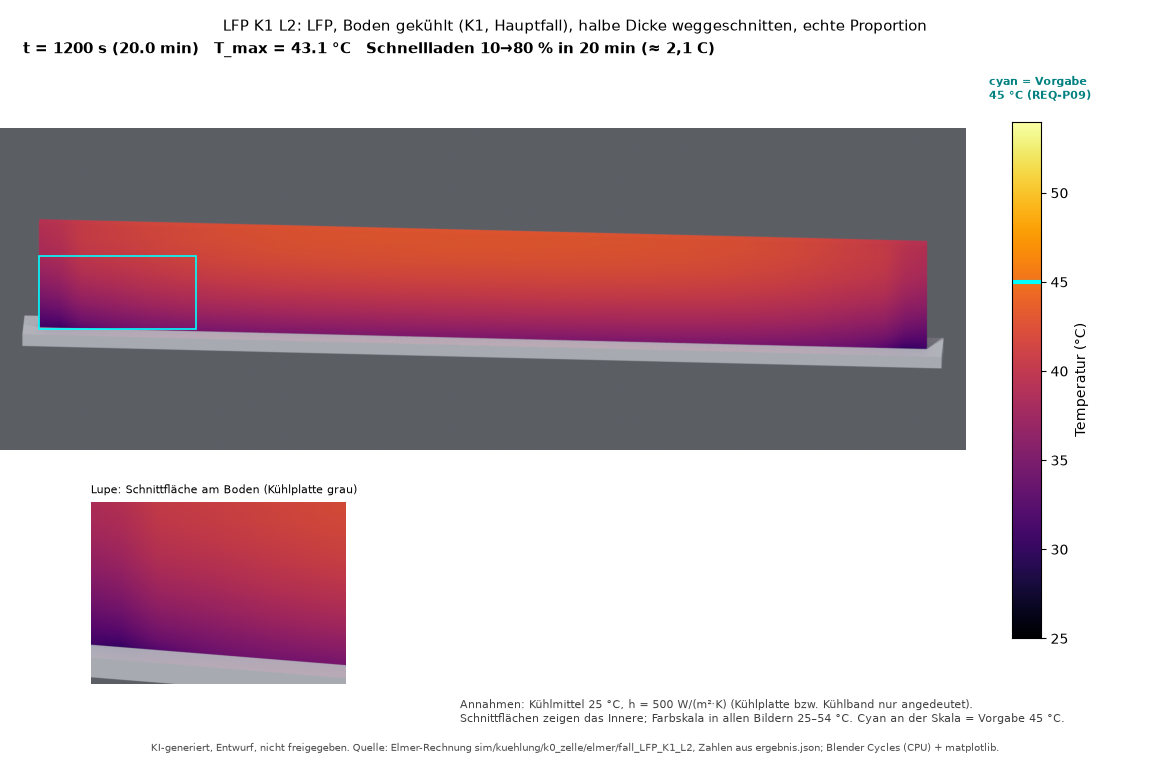
\includegraphics[width=0.49\linewidth]{bilder/k0_cycles_LFP_K1_t1200.png}\hfill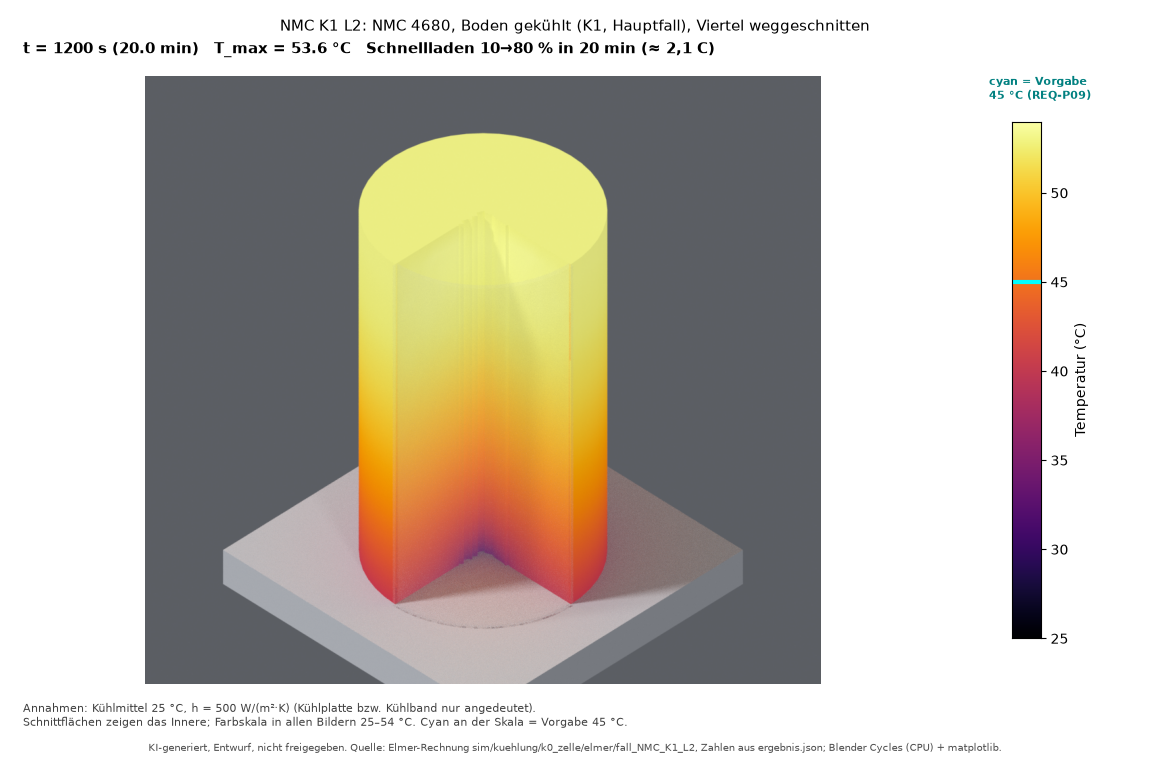
\includegraphics[width=0.49\linewidth]{bilder/k0_cycles_NMC_K1_t1200.png}
\caption[]{K0 nach 1200 s Schnellladen, Boden gekühlt: LFP (links, T$_{\max}$ 43,1 °C) und 4680 (rechts, T$_{\max}$ 53,6 °C). Quelle: \path{sim/kuehlung/k0_zelle/bilder/cycles_LFP_K1_L2_t1200.png}, \path{cycles_NMC_K1_L2_t1200.png}; Zahlen \path{sim/kuehlung/k0_zelle/ergebnis.json}.}\end{figure}
\lesehilfe{Links die LFP-Zelle in echter Proportion (681 × 90 × 14 mm), die halbe Dicke ist weggeschnitten, unten liegt die Kühlplatte. Die Lupe zeigt die Schnittfläche am Boden. Rechts die 4680-Zelle mit einem weggeschnittenen Viertel; der Boden steht auf der Kühlplatte.
Violett ist kühl, gelb heiß, die türkise Marke an der Skala ist das Zielband 45 °C. Die LFP-Zelle bleibt darunter (43,1 °C), die 4680 liegt fast überall darüber: nur am Boden, wo die Wärme abfließt, ist sie kühler.}
\begin{figure}[H]\centering
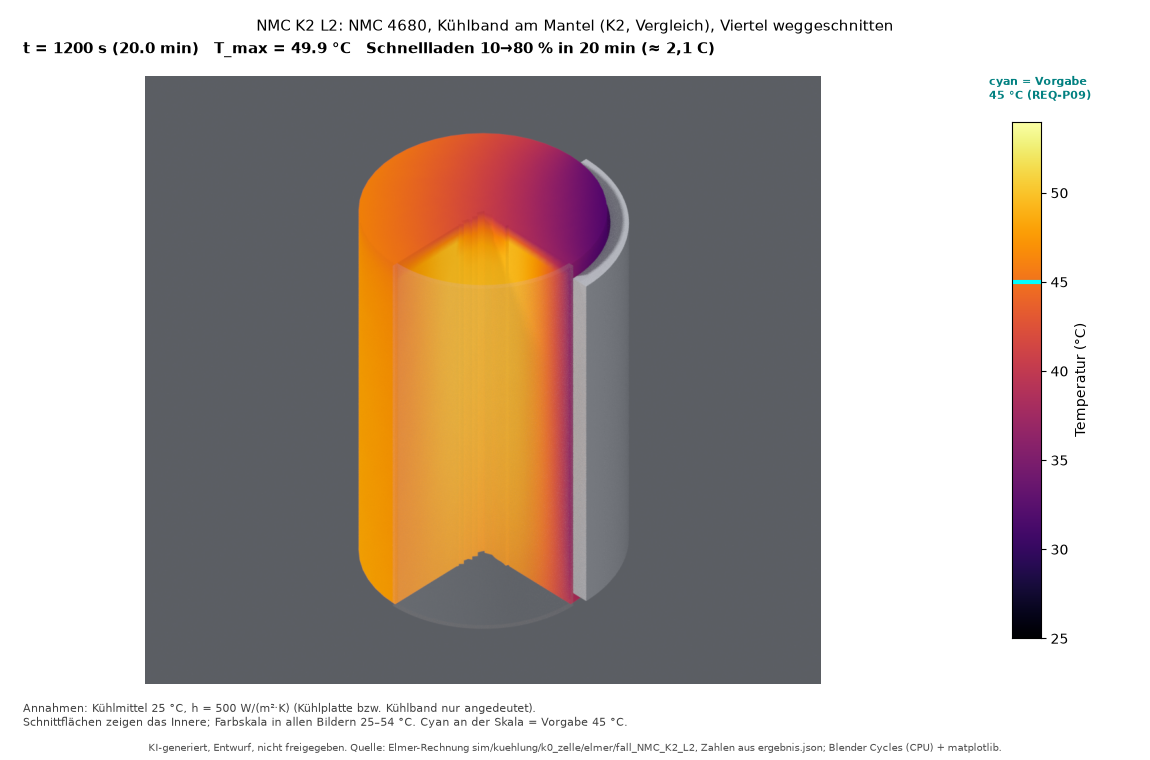
\includegraphics[width=0.62\linewidth]{bilder/k0_cycles_NMC_K2_t1200.png}
\caption[]{K0, 4680 mit Kühlband am Mantel (K2), nach 1200 s Schnellladen, T$_{\max}$ 49,9 °C. Quelle: \path{sim/kuehlung/k0_zelle/bilder/cycles_NMC_K2_L2_t1200.png}.}\end{figure}
\lesehilfe{Wie das 4680-Bild oben, nur kühlt hier ein Band (grau, rechts hinten) über ein Viertel des Umfangs statt des Bodens. Die Seite zum Band ist kühler, die gegenüberliegende bleibt heiß; der Höchstwert 49,9 °C liegt unter dem Fall mit Bodenkühlung, aber immer noch über der Marke 45 °C.}

\subsection*{Abgleich mit der Erwartung und Deutung (Opus)}
\textbf{Abgleich (Sonnet, ERGEBNIS.md):} Wärme, Leitfähigkeit, LFP L1/L2 und die Spreizung 5 K bei L2 (beide verfehlt) wie erwartet. \emph{Verfehlt:} NMC bei 1C 33,5 statt etwa 31 °C und bei L2 53,6 statt 45--50 °C; ebenso K2 mit ΔT 18,1 statt 20 K oder mehr.\quelle{\path{sim/kuehlung/k0_zelle/ERGEBNIS.md}, Abgleich Punkt 3 bis 5}

\textbf{Deutung (Opus, \path{sim/kuehlung/k0_zelle/DEUTUNG.md}):}
\begin{itemize}[nosep]
\item Die verfehlte NMC-Erwartung ist ein Fehler der Erwartung, nicht der Rechnung: Opus hatte den Temperatursprung am Kühlrand (Film Q/(h·A)) vergessen. Der 4680-Boden ist nur 16,6 cm² groß; der Film kostet 4,2 K bei 1C und 18 K bei 2,1C. Mit Film ergibt die Gegenrechnung 34 °C (Rechnung 33,5 °C).
\item Engpass der 4680 ist die kleine Bodenfläche, nicht die Leitung im Wickel. Engpass der LFP ist der Wärmeweg von 90 mm in der Höhe.
\item Mit Kühlung nur von unten ist das Ziel 5 K beim Schnellladen für keine Variante erreichbar. Beim Dauerbetrieb 1C passen beide.
\item Stärkster Hebel ist der Innenwiderstand (grob aus W20 Abb. 8 abgelesen); das Zellmodell C1 bis C3 mit dem Blade-Pulsdatensatz soll ihn schärfen.
\end{itemize}
\textbf{Grenzen des Modells} (Sonnet, ERGEBNIS.md): Wärmequelle gleichmäßig im Kern; Endzonen (Pole, Halter) als reine Luft; W18-Leitfähigkeiten stammen von einer anderen Zelle; Kühlmittel 25 °C und h = 500 W/(m²·K) sind Annahmen; Wärmekapazität des Gehäuses fehlt.
Die offene Frage an den Autor (5 K beim Schnellladen) ist durch K1 beantwortet, siehe unten.


\subsection*{K1: Schnellladen, Ladeprofile und Kühlvarianten}
\begriffe{\textbf{Ladeprofil P0 bis P4}: Verlauf des Ladestroms über die Zeit (P0 konstant 2,1C, P1 Stufen, P2 Puls, P3 und P4 begrenzter Strom bei 25 bzw. 30 min). \textbf{C-Rate}: 1C lädt die Zelle in einer Stunde.
\textbf{K3}: Kühlplatte oben und unten. \textbf{K1b}: 4680 oben über Zellverbinder und Isolierpad gekühlt. \textbf{$h_\mathrm{eff}$}: Ersatz-Wärmeübergang des Kühlrands. \textbf{Spreizung}: Temperaturunterschied im Zellkern.}
\kasten{Stand.}{K1 und K1b sind mit Elmer gerechnet (Fortsetzung von K0). Zahlen aus \texttt{sim/kuehlung/k1\_schnellladen/ergebnis.json}; die Deutung stammt von Opus und ist gekennzeichnet. Alle Randwerte
(Kühlmittel 25 °C, $h$ = 500 W/(m²·K), Innenwiderstand) sind \emph{Annahmen} wie in K0.}
Fragestellung (Auftrag Opus): Welche Ladeprofile und welche Kühlung erfüllen beim Schnellladen die Vorgaben 45 °C und 5 K? Die Wärme folgt $Q(t) = I(t)^2 \cdot R$.
\textbf{Prüfungen:} P0 reproduziert K0 L2 bei LFP auf 0,0000 K; bei NMC weicht es um $-0{,}21$ K (T$_{\max}$) bzw. $-0{,}35$ K ($\Delta$T) ab, weil das NMC-Netz nach dem Nachtrag das aktuelle CAD (Kernloch r 6,25 mm) verwendet. Das
Wärmeintegral stimmt mit den Stufenprofilen auf höchstens 0,34 \% überein.\quelle{\path{sim/kuehlung/k1_schnellladen/ERGEBNIS.md}, Abschnitte 1, 3 und 7; \path{DEUTUNG.md}}

\bild{k1_profile.png}{0.82}{K1: die fünf Ladeprofile P0 bis P4 (Strom oben, Ladezustand unten). Quelle: \path{sim/kuehlung/k1_schnellladen/profile.png}.}
\lesehilfe{Oben der Ladestrom in C (1C lädt in einer Stunde voll, 2C in 30 Minuten), unten der Ladezustand von 10 auf 80 \%. Alle fünf Profile laden denselben Hub, aber P0 in 20 Minuten mit konstant 2,1C, P1 in Stufen (3C, 2C, 1,385C), P2 mit Puls (4,2C an, dann aus, Takt 60 s), P3 mit 1,68C in 25 Minuten und P4 mit 1,4C in 30 Minuten.
Je höher der Strom, desto mehr Wärme (sie wächst mit dem Quadrat des Stroms). Hier gibt es kein Zielband, nur die Lade-Endmarke 80 \% (grün gestrichelt).}

\textbf{Ergebnisse.}
\begin{center}\small
\begin{tabular}{@{}lccccc@{}}\toprule
 & \multicolumn{2}{c}{LFP} & \multicolumn{2}{c}{NMC (4680)} & Vorgaben\\
Fall (Start 25 °C, $h$ = 500 wenn nicht anders) & T$_{\max}$ °C & $\Delta$T K & T$_{\max}$ °C & $\Delta$T K & LFP / NMC\\\midrule
P0 konstant 2,1C, 20 min (= K0 L2) & 43,1 & 10,6 & 53,4 & 15,7 & nur T / keine\\
P1 Stufen 3C/2C/1,38C, 20 min & 44,1 & 11,3 & 54,9 & 16,6 & nur T / keine\\
P2 Puls 4,2C an/aus, 20 min & 61,7 & 21,3 & 82,5 & 31,6 & keine / keine\\
P3 konstant 1,68C, 25 min & 37,5 & 7,4 & 44,9 & 11,0 & nur T / nur T\\
P4 konstant 1,4C, 30 min & 34,1 & 5,4 & 39,6 & 8,1 & nur T / nur T\\
P0, Boden h 1000 & 39,7 & 10,8 & 49,0 & 17,3 & nur T / keine\\
P0, Boden h 2000 & 37,4 & 10,5 & 46,0 & 17,8 & nur T / keine\\
P0, Start und Kühlmittel 15 °C & 33,1 & 10,6 & 43,4 & 15,7 & nur T / nur T\\
P0, Kühlplatte oben und unten (K3) & 33,8 & 4,6 & 38,9 & 5,8 & beide / nur T\\
P1, K3 & 37,6 & 6,3 & 44,3 & 8,0 & nur T / nur T\\
P0, K3, h 1000 & 30,8 & 3,8 & 34,6 & 5,7 & beide / nur T\\
P3, K3 & – & – & 34,0 & 3,8 & – / beide\\
P3, Boden h 2000 & – & – & 39,0 & 11,9 & – / nur T\\
P0, K1b oben über Verbinder und Pad & – & – & 42,8 & 8,1 & – / nur T\\
P3, K1b & – & – & 36,8 & 5,4 & – / nur T\\
P4, K1b & – & – & 33,3 & 3,8 & – / beide\\
\bottomrule\end{tabular}\end{center}
\tquelle{Spitzenwerte über die Ladezeit; \path{sim/kuehlung/k1_schnellladen/ergebnis.json}, Felder T\_max\_Spitze\_C und dT\_Spitze\_K (Tabelle mit Ladeende, Zeiten über der Schwelle und Wärmeintegral: \path{ERGEBNIS.md} Abschnitt 2). „beide“ = T$_{\max}$ ≤ 45 °C und $\Delta$T ≤ 5 K (REQ-P09). „–“: nicht gerechnet.}

\bild{k1_landkarte.png}{0.92}{K1: Landkarte aller gerechneten Fälle gegen REQ-P09. Quelle: \path{sim/kuehlung/k1_schnellladen/landkarte.png}.}
\lesehilfe{Jede Zeile ist ein Fall, jede Spalte ein Spitzenwert. Grün heißt Vorgabe eingehalten (T$_{\max}$ ≤ 45 °C bzw. $\Delta$T ≤ 5 K), rot verfehlt, grau nicht gerechnet. Die Spalte „Ampel“ fasst beide Vorgaben zusammen: grün beide erfüllt, gelb nur eine, rot keine.
Die grünen Felder in der Ampel sind: LFP mit Kühlplatte oben und unten (mit h 500 und h 1000) sowie NMC mit K3 bei 25 min (Deckel direkt gekühlt), mit K1b bei 30 min und mit K1b bei 25 min und höherer Bedeckung.}
\bild{k1_verlauf_kuehlung_LFP.png}{0.88}{K1: LFP, Temperatur und Spreizung je Kühlfall (Profil P0). Quelle: \path{sim/kuehlung/k1_schnellladen/verlauf_kuehlung_LFP.png}.}
\lesehilfe{Oben die höchste Temperatur in der Zelle über die Ladezeit, unten der Temperaturunterschied im Kern. Der grüne Bereich ist das \emph{Zielband} (unterhalb der beschrifteten Linie 45 °C bzw. 5 K). Mehr Wärmeübergang am Boden (h 1000, h 2000) und Vorkühlung (V15) senken nur die Höchsttemperatur; die Spreizung bleibt bei etwa 10 K. Erst die Kühlung von zwei Seiten (K3) bringt die Spreizung in das grüne Band.}
\bild{k1_verlauf_kuehlung_NMC.png}{0.88}{K1: 4680, Temperatur und Spreizung je Kühlfall (Profil P0, wenn nicht anders). Quelle: \path{sim/kuehlung/k1_schnellladen/verlauf_kuehlung_NMC.png}.}
\lesehilfe{Wie das LFP-Bild, für die 4680-Zelle; zusätzlich die Fälle mit Profil P3 und die Kühlung oben über Verbinder und Pad (K3b, gepunktet). Zielband grün, Linien 45 °C und 5 K. Bei Kühlung nur am Boden (h 1000, h 2000) steigt die Spreizung sogar leicht, weil der Boden kühler wird, während die Kernspitze bleibt.
Nur die beidseitig gekühlten Fälle mit geringerem Strom (P3, 25 min) liegen im Band.}

\textbf{K1b: 4680 oben über Verbinder und Isolierpad.} Bei der Rundzelle sitzt oben der Zellverbinder (Al, 1,5 mm), darüber ein elektrisch isolierendes Pad (ENT-095, entschieden; Dicke 1 mm ist Annahme) und die obere Kühlplatte. K1b modelliert das als Ersatz-Wärmeübergang
$h_\mathrm{eff} = \varphi / (1/h + t_\mathrm{pad}/k_\mathrm{pad} + t_\mathrm{v}/k_\mathrm{v})$ mit Bedeckung $\varphi$ = 0,5 (Band 0,3 bis 0,7), Pad $k_\mathrm{pad}$ 3 W/(m·K) (Band 1 bis 6), das ergibt $h_\mathrm{eff}$ = 213,7 W/(m²·K)
(alles Annahme Opus). Ergebnis: P0 (20 min) 42,8 °C und 8,1 K, P3 (25 min) 36,8 °C und 5,4 K, \textbf{P4 (30 min) 33,3 °C und 3,8 K} (beide Vorgaben erfüllt). Empfindlichkeit bei P3: mit $\varphi$ = 0,7 4,7 K (erfüllt), mit $\varphi$ = 0,3 6,6 K, mit $k_\mathrm{pad}$ 1 6,0 K,
mit $k_\mathrm{pad}$ 6 5,2 K.\quelle{\path{sim/kuehlung/k1_schnellladen/ERGEBNIS.md}, Abschnitt 8; \path{ergebnis.json} (NMC\_P0\_K3b, NMC\_P3\_K3b, NMC\_P4\_K3b, ...\_phi03, ...\_phi07, ...\_kpad1, ...\_kpad6)}
Auf dieser Grundlage hat der Autor für die 4680 die Ladezeit 30 min festgelegt (REQ-P05).\quelle{\path{docs/01_lastenheft.md}, REQ-P05; \path{sim/kuehlung/TABELLEN_TEMPERATUR.md}, Abschnitt Folge}

\textbf{Deutung (Opus, \path{sim/kuehlung/k1_schnellladen/DEUTUNG.md}):}
\begin{itemize}[nosep]
\item \textbf{LFP:} Beidseitige Kühlung (K3) erfüllt bei 20 min beide Vorgaben (33,8 °C und 4,6 K; mit h 1000 30,8 °C und 3,8 K). Alternativ Begrenzung auf 30 min: 34,1 °C und 5,4 K, also knapp verfehlt.
\item \textbf{Stufenladen} bringt thermisch nichts (LFP 44,1 °C / 11,3 K gegen 43,1 / 10,6 bei P0); \textbf{Puls bzw. Zellen im Wechsel} verschlechtert stark (LFP 61,7 °C / 21,3 K), wie vorab aus $\int I^2 \mathrm{d}t$ erwartet.
\item \textbf{Bessere Kühlung (h) und Vorkühlung} senken nur T$_{\max}$, nicht die Spreizung. Bei der 4680 steigt $\Delta$T mit h leicht.
\item \textbf{NMC mit Tab-Scheibe:} NMC K3 bei P0 38,9 °C / 5,8 K (knapp verfehlt), bei P3 (25 min) 34,0 °C / 3,8 K. Die Ersatzleitfähigkeit des 3,6-mm-Spalts ($k_z$ 31 W/(m·K)) ist die stärkste neue Annahme (Sonnet). Der erste Lauf (47,9 °C / 12,3 K) war nicht belastbar, siehe Kapitel~\ref{k:fehler}, Zeile 12.
\item \textbf{Erwartungsfehler (Opus):} Zeitkonstanten unterschätzt (P1-Spitze erst bei 810 s; NMC P3/P4 kühler als erwartet).
\end{itemize}
\textbf{K1b-Deutung:} liegt als Opus-Deutung nicht vor; die Bewertung oben folgt der Sonnet-Auswertung gegen die Erwartung (Erwartung P4 etwa 35 °C / 4,5 bis 5 K, Ergebnis 33,3 °C / 3,8 K).\quelle{\path{sim/kuehlung/k1_schnellladen/ERGEBNIS.md}, Abschnitt 8}
\kasten{Folge für Auslegung (Entscheidungen des Autors, 2026-11-17).}{Kühlplatte oben und unten (ENT-088); Schnellladen LFP 20 min, NMC 30 min (REQ-P05). Offen bleibt die Annahme zum oberen Kühlpfad der 4680 (Pad, Bedeckung $\varphi$).\quelle{\path{sim/kuehlung/TABELLEN_TEMPERATUR.md}, Abschnitt Folge}}


%======================================================================
\section{Gehäuse und Pack}\label{k:pack}
\begriffe{\textbf{Querträger}: Hohlprofil quer zur Fahrtrichtung, das Seitenlast über die Packbreite leitet. \textbf{Seitenrahmen}: umlaufendes Profil. \textbf{Kühlplatte}: Platte mit Kühlkanälen, hier oben und unten (ENT-088).
\textbf{Wärmeleitpad}: weiche, wärmeleitende Schicht zwischen Zelle und Kühlplatte. \textbf{Zellträger} und \textbf{Verguss}: Kunststoffteil und Schaum, die die Rundzellen halten. \textbf{Hüllkörper}: Zelle als einfacher Block ohne Innenleben. \textbf{CTP}: Cell-to-Pack, Zellen ohne Modulgehäuse.}
\kasten{Stand.}{M0 (Höhe und Länge) und G4 (Pack-CAD in FreeCAD) sind gerechnet bzw. gebaut und von Opus an Stichproben geprüft. Maße kommen aus entschiedenen Akten und aus \emph{vorgeschlagenen} Akten (Entwurf); Dichten und Füllgrade sind Annahmen (Opus).
Zahlen: \path{sim/mechanik/m0_gehaeuse/ergebnis.json}, \path{cad/pack/entwurf/ergebnis*.json}.}

\subsection*{Recherche W21 und W22: Bauweise, Querträger, Seitenlast}
W21 (Gehäuse, Zitatprüfung 12 bestätigt, 0 Fehler) liefert die Bauweise (CTP, Wanne, Deckel und Rahmen aus Aluminium), aber keine Maße. W22 (Zitatprüfung 13 bestätigt, 1 Fehler) liefert nach Lauf 3 die Maße der Querträger aus einem Patent (US9045030B2, Pack 2,7 × 1,5 m):
Profil 54 × 26 mm, Oberprofil 19 × 30 mm, Wand 2 bis 3 mm; Seitenlast etwa 600 kN bei Fahrzeugen über 2600 kg; Alu-Strangpressprofil mehr als 20 \% leichter als Stahl (US20200148066A1).
\textbf{Gesperrt} ist der SSAB-Wert „1,8 mm“ Blechdicke (das Zitat fehlte zweimal im Quelltext). Die Seitenrahmenbreite hat weiter keinen Beleg (30 mm ist Entscheidung des Autors, ENT-087).\quelle{\path{forschung/ergebnis/W21.pruefung.txt}, \path{W22.pruefung.txt}; \path{BEFUNDE.md} (Eintrag W21/W22 Verstrebungen)}
Die 600 kN gelten für über 2600 kg und sind nicht auf 1500 kg skaliert; sie sind Hinweis, kein Lastfall.

\subsection*{Herstellervergleich Rundzellen (W24 bis W26)}
Haiku hat aus den geprüften Recherchen eine Vergleichstabelle zusammengestellt (mechanisch, ohne Deutung). Auswahl der für Gehäuse und Pack nützlichen Zeilen:
\begin{center}\small\begin{tabularx}{\linewidth}{@{}p{4.2cm}Xp{1.6cm}@{}}\toprule
\textbf{Größe} & \textbf{Wert (Quelle in der Tabelle: URL aus W24 bis W26)} & \textbf{Thema}\\\midrule
Tesla 4680, Maße und Masse & 46 × 80 mm, 0,355 kg & W24\\
Gehäusewand Tesla 4680 & 0,5 bis 0,6 mm (Akte ENT-029 setzt 0,4 mm nach W20 Tab. 1; Abweichung offen) & W24, W25\\
Ladezeit 0 auf 80 \% (Model Y) & etwa 30 min & W25\\
Zellmontage (Lucid, Rivian, Tesla) & einseitig kontaktiert & W26\\
Kühlung Tesla & Potting zwischen Zelle und Kühlsystem, zum Anbinden und Schutz & W26\\
Lucid Air Pack & 220 S / 30 P, 118 kWh; Busbar Al, 1/5 des Gesamtstroms je Busbar; Bodenplatte 8 mm (Verbund) & W26\\
BMW 800-V-System & 350 kW DC-Schnellladeleistung & W26\\\bottomrule\end{tabularx}\end{center}
\tquelle{\path{forschung/vergleich_rundzellen.md} (Auszug); Quellen \path{forschung/ergebnis/W24.md}, \path{W25.md}, \path{W26.md} (24, 10 und 14 bestätigte Belege, je 0 Fehler). P14 lieferte 0 Belege (HTTP 503), keine Zeile übernommen.}

\subsection*{M0: Höhe und Länge des Gehäuses}
M0 stapelt die Schichten (Unterfahrschutz 3, Luft 5, Boden 3, Kühlplatte unten 8, Pad 1, Zelle, Pad 1, Kühlplatte oben 8, Deckel 2 mm) und prüft Höhe, Länge und Plätze.
Ergebnis: Höhe LFP 121 mm (Zelle 90 mm, Rest 9 mm bis zur Grenze 130 mm \annahme), NMC 111 mm (Zelle 80 mm, Rest 19 mm). Länge LFP: Zellstapel 1874 mm, netto 1964 mm, Gehäuse 2024 mm (die Akte ENT-102 setzt 2030 mm);
der Zuwachs gegen 1950 mm kommt von den drei Querträgern. NMC: 1120 Plätze (ohne Querträger 1260, Verlust 140 durch die Träger), benötigt 868, Belegung 77,5 \%; Länge 1950 mm reicht. Querträger 400 mm², je 1,48 kg, zusammen 4,44 kg.
Alle Punkte der Erwartung sind erfüllt.\quelle{\path{sim/mechanik/m0_gehaeuse/ergebnis.json}; \path{ERGEBNIS.md} Abgleich Punkt 1 bis 5}
\begin{figure}[H]\centering
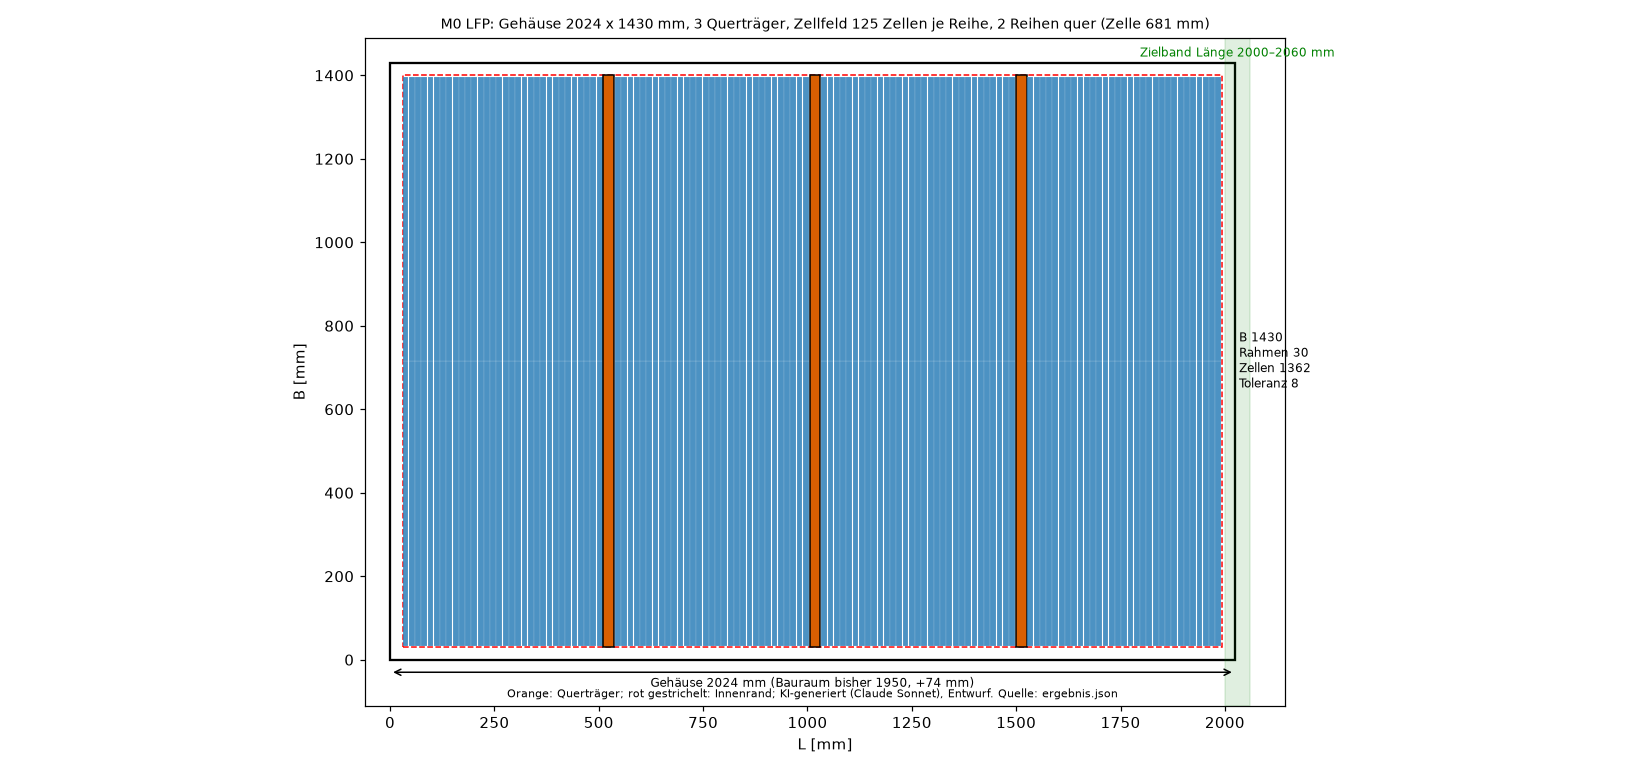
\includegraphics[width=0.49\linewidth]{bilder/m0_draufsicht_LFP.png}\hfill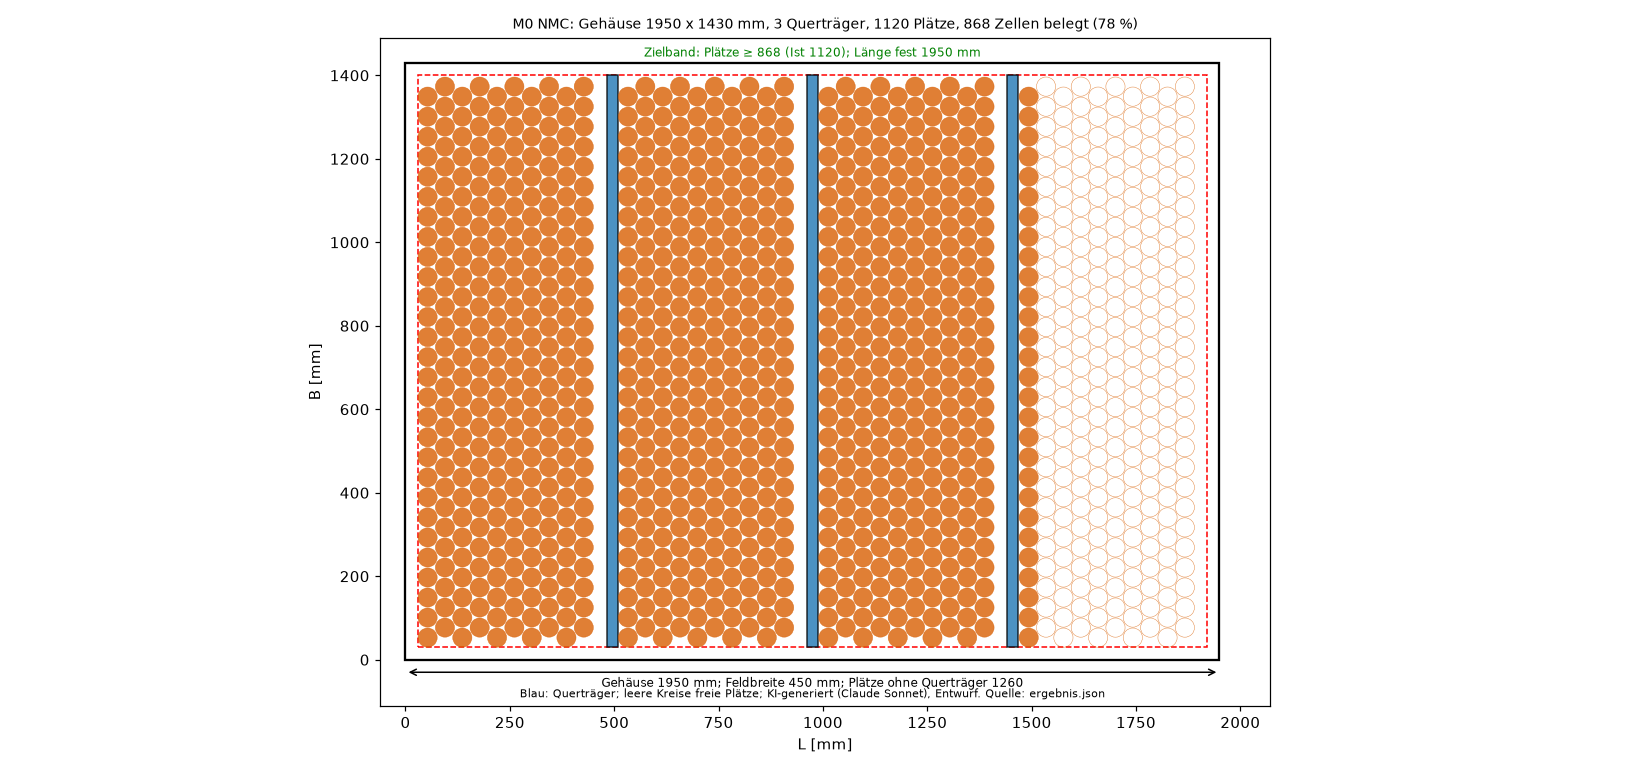
\includegraphics[width=0.49\linewidth]{bilder/m0_draufsicht_NMC.png}
\caption[]{M0, Draufsicht auf das Gehäuse: LFP (links, Länge 2024 mm im Zielband 2000 bis 2060 mm) und NMC (rechts, 1120 Plätze gegen 868 benötigte). Quelle: \path{sim/mechanik/m0_gehaeuse/draufsicht_LFP.png}, \path{draufsicht_NMC.png}.}\end{figure}
\lesehilfe{Blick von oben. Links die LFP-Zellen als dünne blaue Streifen in zwei Reihen, dazwischen die drei orangen Querträger; die schwarze Linie ist die Außenkante, rot gestrichelt der Innenrand, das grüne Band das \emph{Zielband} der Länge (2000 bis 2060 mm). Rechts die runden 4680-Zellen im Wabenmuster in vier Feldern zwischen den Querträgern;
gefüllte Kreise sind belegte Plätze, leere sind frei. Ziel: mindestens 868 belegte Plätze.}
\begin{figure}[H]\centering
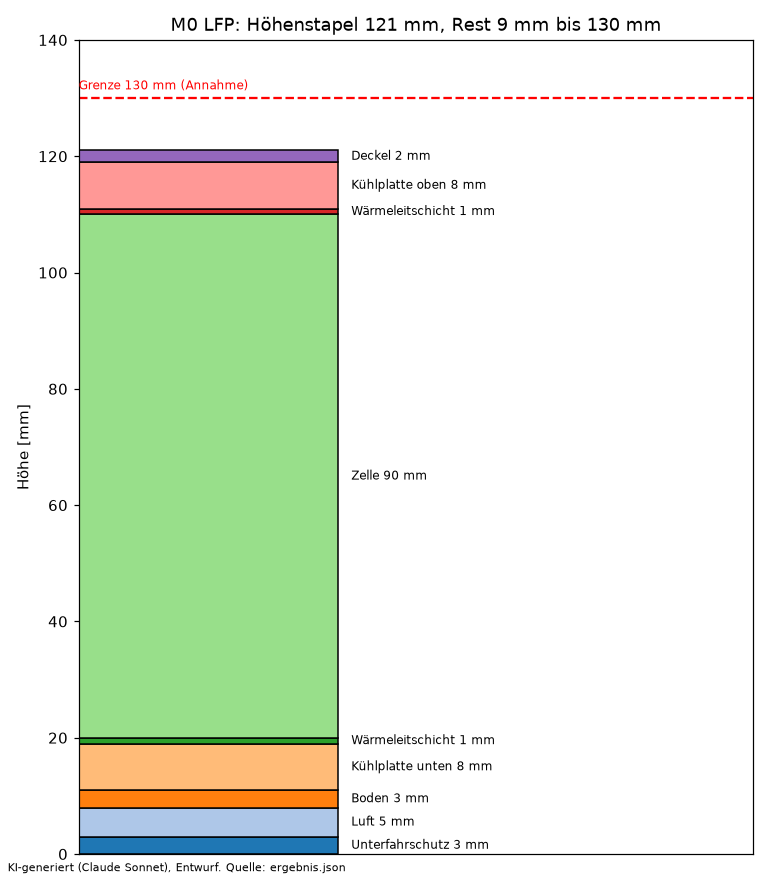
\includegraphics[width=0.40\linewidth]{bilder/m0_schnitt_LFP.png}\hfill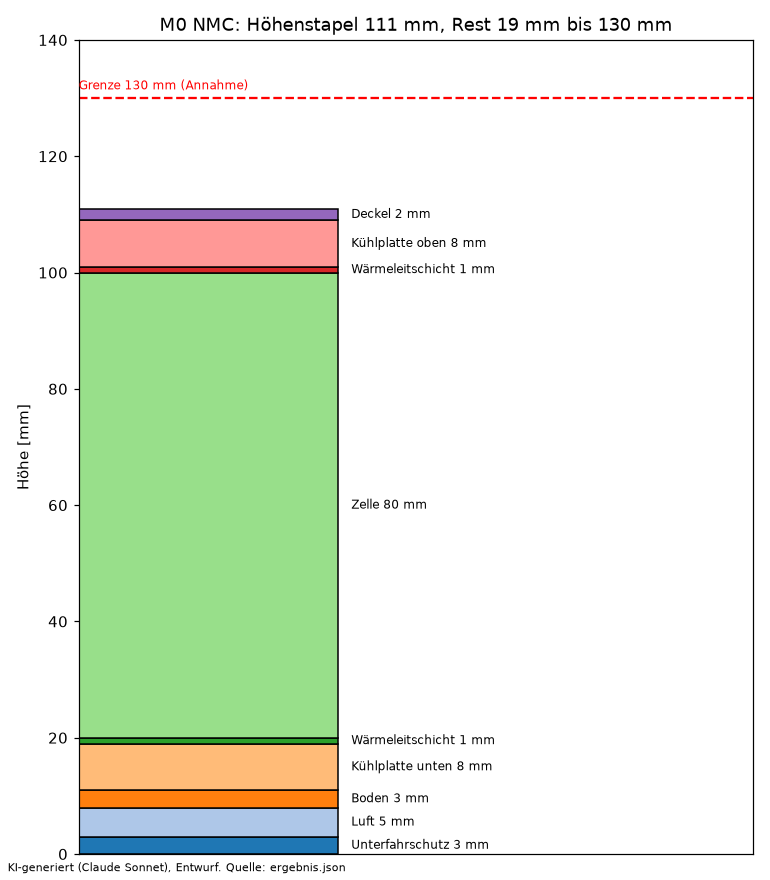
\includegraphics[width=0.40\linewidth]{bilder/m0_schnitt_NMC.png}
\caption[]{M0, Höhenstapel: LFP 121 mm (links) und NMC 111 mm (rechts) gegen die Grenze 130 mm (Annahme). Quelle: \path{sim/mechanik/m0_gehaeuse/schnitt_LFP.png}, \path{schnitt_NMC.png}.}\end{figure}
\lesehilfe{Seitenschnitt als Stapel von unten (Unterfahrschutz) nach oben (Deckel), jede Schicht mit ihrer Dicke in Millimetern. Die rote gestrichelte Linie ist die Höhengrenze 130 mm (Annahme). Beide Stapel liegen darunter; die Zelle ist bei beiden die dickste Schicht.}

\subsection*{G4: Pack-CAD (Freigabestand)}
G4 baut beide Packs in FreeCAD aus den Akten (entschiedene und vorgeschlagene) und prüft Kollisionen und Masse. Stand \emph{Freigabestand}: Der Autor hat ENT-096 bis 101 freigegeben und für die NMC-Variante ein eigenes Gehäuse von 1950 mm (ENT-103; LFP 2030 mm, ENT-102) entschieden.
\begin{center}\small
\begin{tabular}{@{}lrr@{}}\toprule
 & LFP & NMC\\\midrule
Gehäuse L × B × H (mm) & 2030 × 1430 × 121 & 1950 × 1430 × 115\\
Zellen & 250 (2 × 125) & 868 (4 Felder × 217)\\
Querträger (Lage in x, mm) & 514, 1008, 1502 & 482, 962, 1442\\
Kollisionen / geprüfte Paare & 0 / 385 & 0 / 5379\\
Masse, Teile mit bekannter Masse (kg) & 611,9 & 473,4\\
Zielband der Erwartung (kg) & 560 bis 620 (erfüllt) & 390 bis 430 (\emph{verfehlt})\\
Abweichung gegen C0b Fall A (616 / 411 kg) & $-0{,}7$ \% & $+15{,}2$ \%\\
Schwerpunkt, Abweichung von der Mitte x / y (mm) & $-1{,}4$ / $-0{,}0$ & $-12{,}3$ / $-11{,}2$\\\bottomrule
\end{tabular}\end{center}
\tquelle{\path{cad/pack/entwurf/ergebnis_LFP.json}, \path{ergebnis_NMC.json}, \path{ergebnis.json}; \path{cad/pack/ERGEBNIS.md}, Abgleich und Nachtrag Freigabestand. Schwerpunkt-Soll $\pm$ 20 mm: beide erfüllt.}
\textbf{Masse.} Der Erstlauf rechnete Kühlplatten und Seitenrahmen als Vollmaterial (LFP 705,5 kg, NMC 556,5 kg). Nach den Annahmen Opus (Kühlplatten Füllgrad 0,4 mit 2 Blechen je 1,5 mm und Kanalstegen; Seitenrahmen als Mehrkammerprofil mit Wand 2,5 mm und 3 Kammern; Dichten Pad 2500, Zellträger 1200, Verguss 300 kg/m³)
ergeben sich 611,9 kg (LFP) und 473,4 kg (NMC). Die Kühlplatten wiegen je Pack 46,6 kg, die Seitenrahmen 21,7 kg (LFP) bzw. 20,1 kg (NMC).\quelle{\path{cad/pack/ERGEBNIS.md}, Nachtrag Massenannahmen}
Dass die NMC-Masse 15,2 \% über C0b liegt, ist ein offener Punkt für Opus. Die Höhe der NMC liegt 4 mm über der M0-Zahl (115 statt 111 mm), weil Zellabgriffe (1 mm) und Gruppenverbinder (3 mm) über der Zelle in M0 nicht im Stapel standen.
Das eigene NMC-Gehäuse von 1950 mm spart gegenüber dem Gehäuse auf LFP-Maß (2030 mm) nur 7 kg (Opus hatte 15 bis 25 kg geschätzt, Kapitel~\ref{k:fehler}).\quelle{\path{docs/08_ki_einsatz_protokoll.md} (G4-Zeilen); \path{bericht/AUFTRAG_BERICHT_02.md}}
\textbf{Annahmen des Modells} (Auszug, \path{cad/pack/ERGEBNIS.md}): LFP-Zellen als Hüllkörper ohne Pole, Reihenverbinder 25 × 3 mm nur am äußeren Zellende; NMC-Gruppenverbinder je 4 Zellen mit Reihenbrücke, Zellabgriffe als Scheiben Ø 12 × 1 mm; Zellträger 2,5 mm (Annahme); Verbinder als Aluminium (Kupfer offen).

\bild{g4_pack_massen.png}{0.85}{G4: Packmasse aus CAD-Volumen, beide Varianten. Quelle: \path{cad/pack/entwurf/pack_massen.png}.}
\lesehilfe{Zwei gestapelte Säulen: links LFP, rechts NMC; Farben zeigen den Anteil der Bauteile (Zellen blau, Kühlplatten türkis, Rahmen, Boden, Deckel und Unterfahrschutz grau, Querträger orange, Verbinder rot). Das grün schraffierte Rechteck ist das \emph{Zielband} der Erwartung, die gestrichelte schwarze Linie die Masse aus der Chemierechnung C0b.
LFP (612 kg) liegt im Band; die NMC-Säule (473 kg) ragt darüber, die Erwartung ist also verfehlt. Kühlplatten-Füllgrad und Rahmenprofil sind Annahmen.}

\begin{figure}[H]\centering
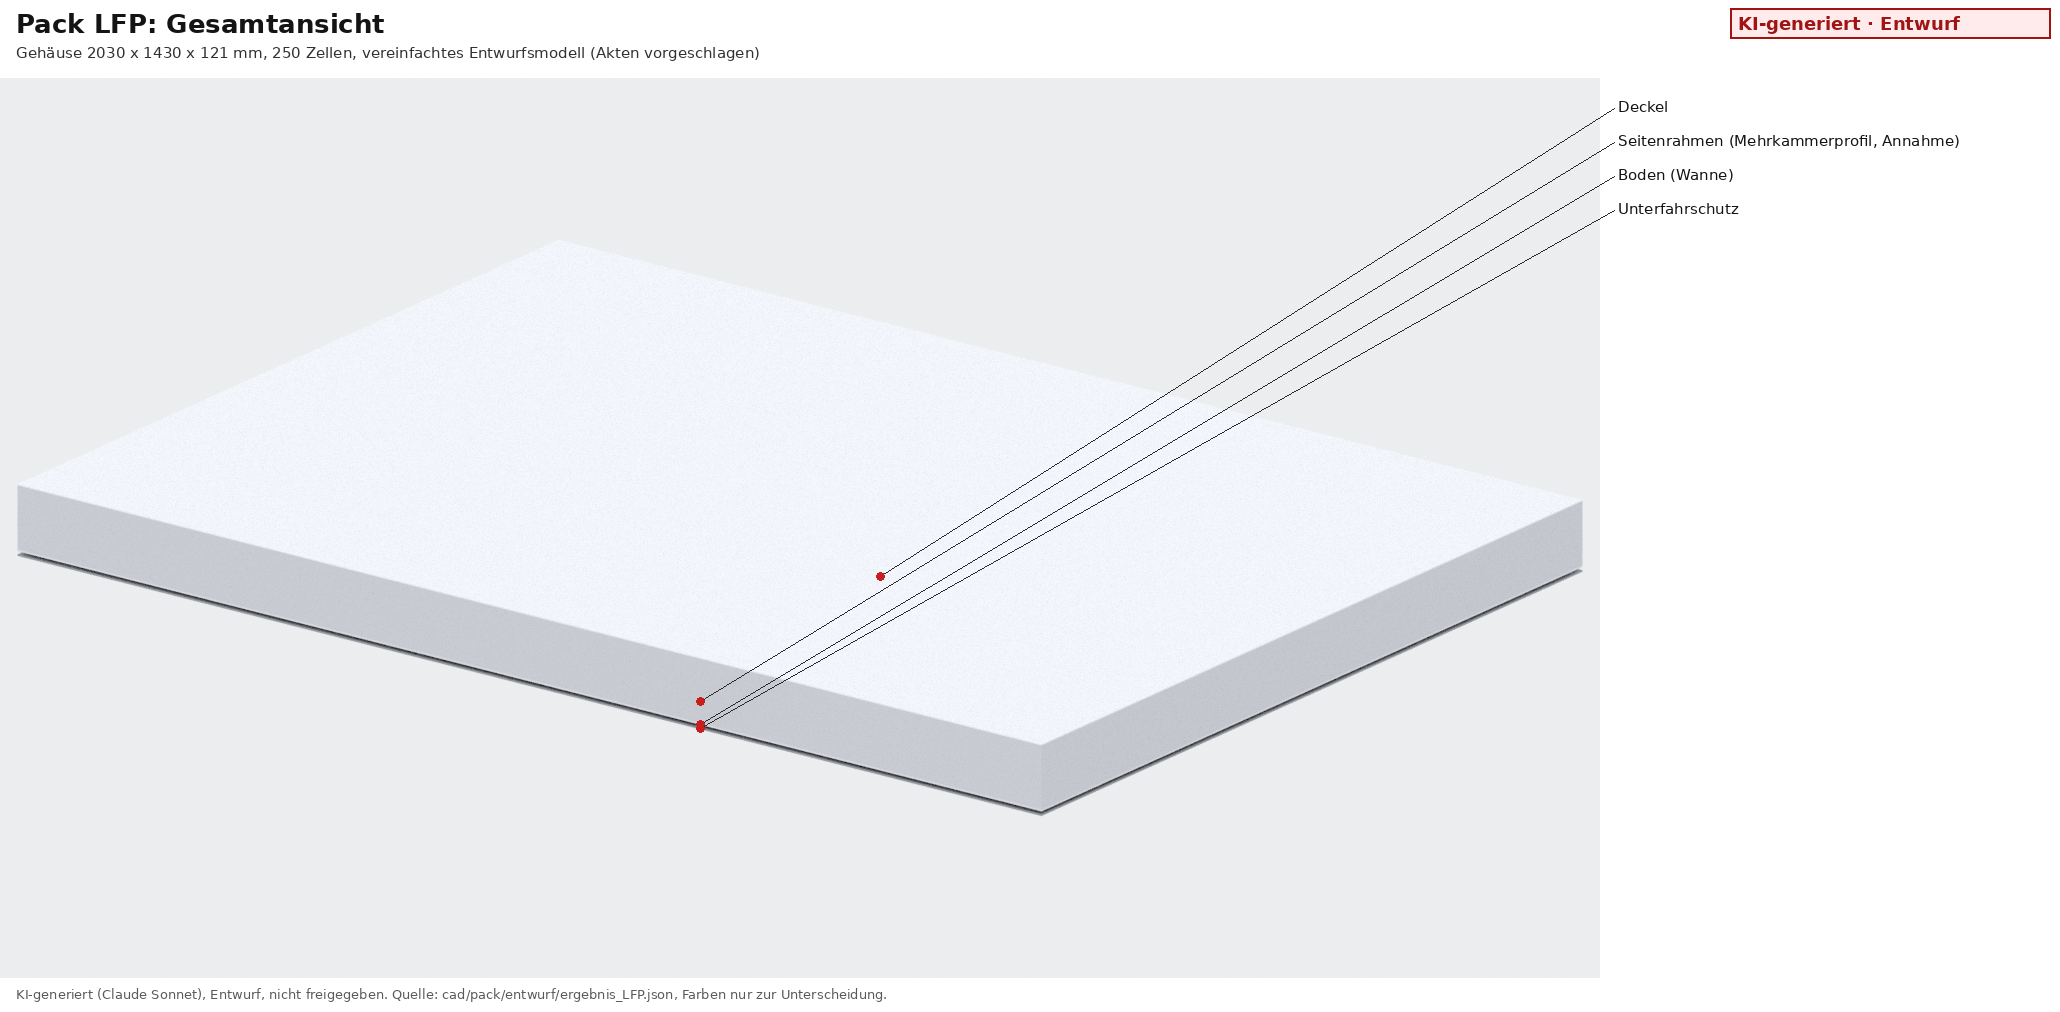
\includegraphics[width=0.49\linewidth]{bilder/g4_pack_LFP_gesamt.png}\hfill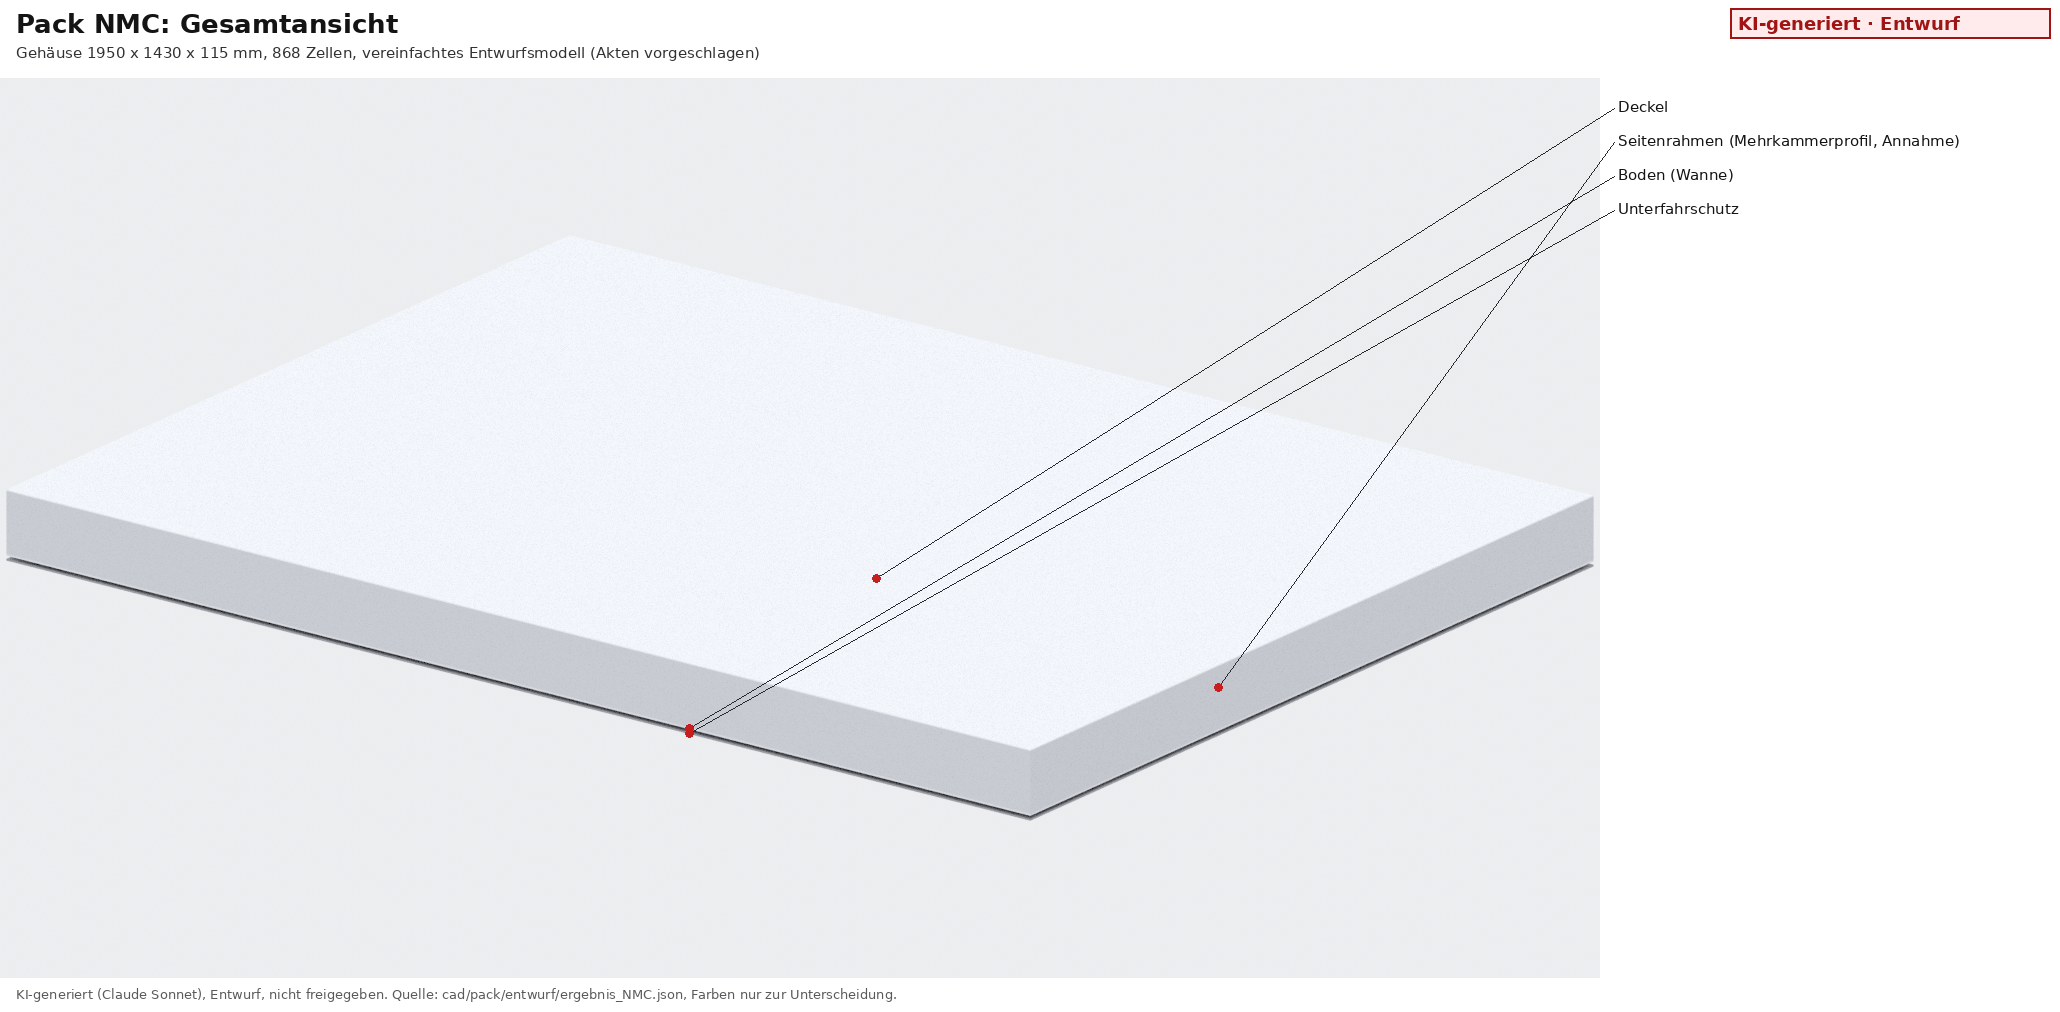
\includegraphics[width=0.49\linewidth]{bilder/g4_pack_NMC_gesamt.png}
\caption[]{G4: Gesamtansicht LFP (links) und NMC (rechts). Quelle: \path{cad/pack/entwurf/pack_LFP_gesamt.png}, \path{pack_NMC_gesamt.png}.}\end{figure}
\lesehilfe{Blick schräg von oben auf das geschlossene Gehäuse (Deckel, Rahmen, Unterfahrschutz); die Maße stehen im Bildtitel. Es ist ein vereinfachtes Entwurfsmodell, nur die Außenform ist zu sehen.}
\begin{figure}[H]\centering
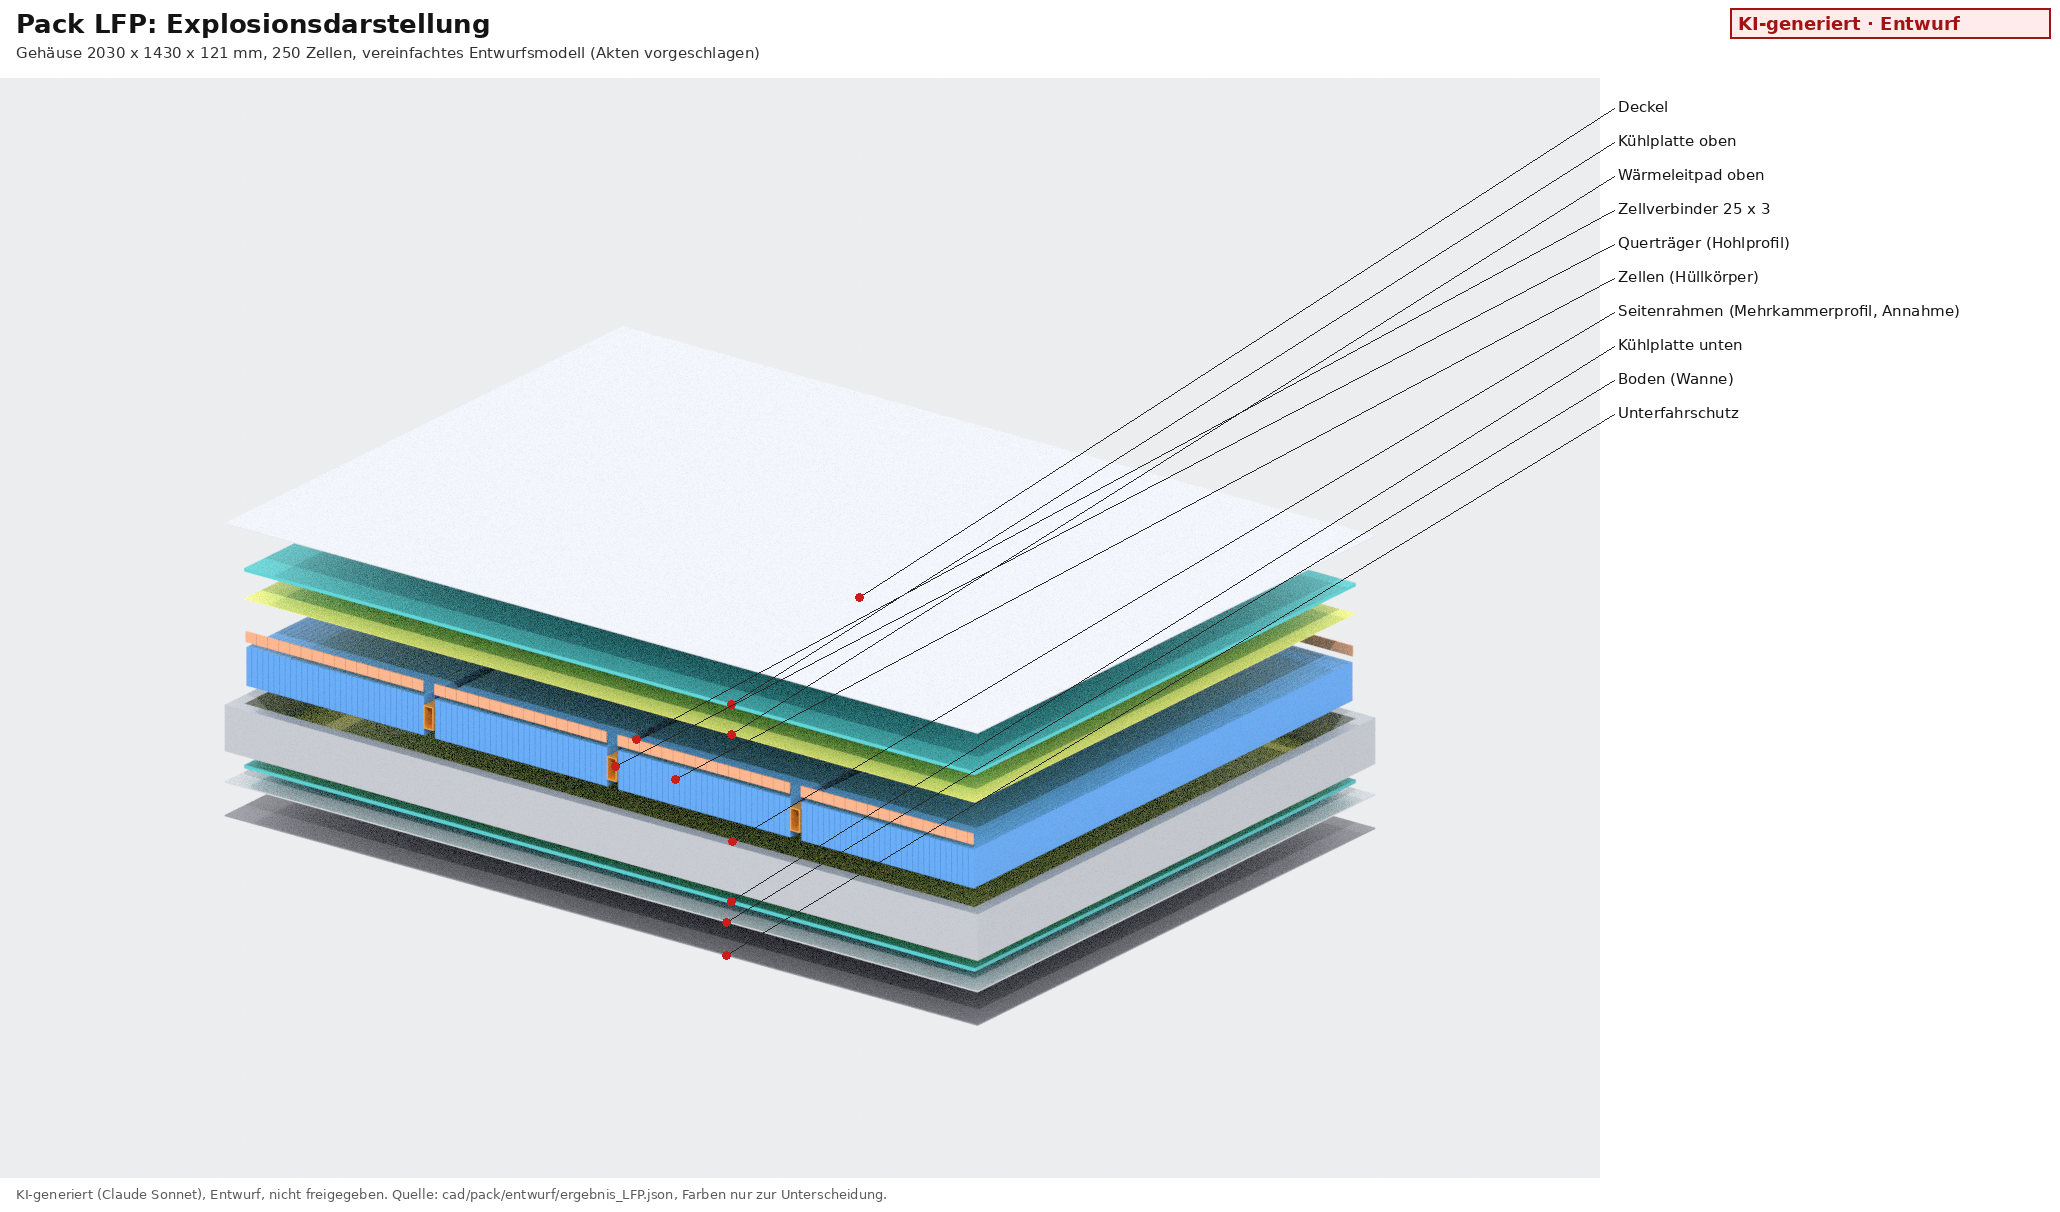
\includegraphics[width=0.49\linewidth]{bilder/g4_pack_LFP_explosion.png}\hfill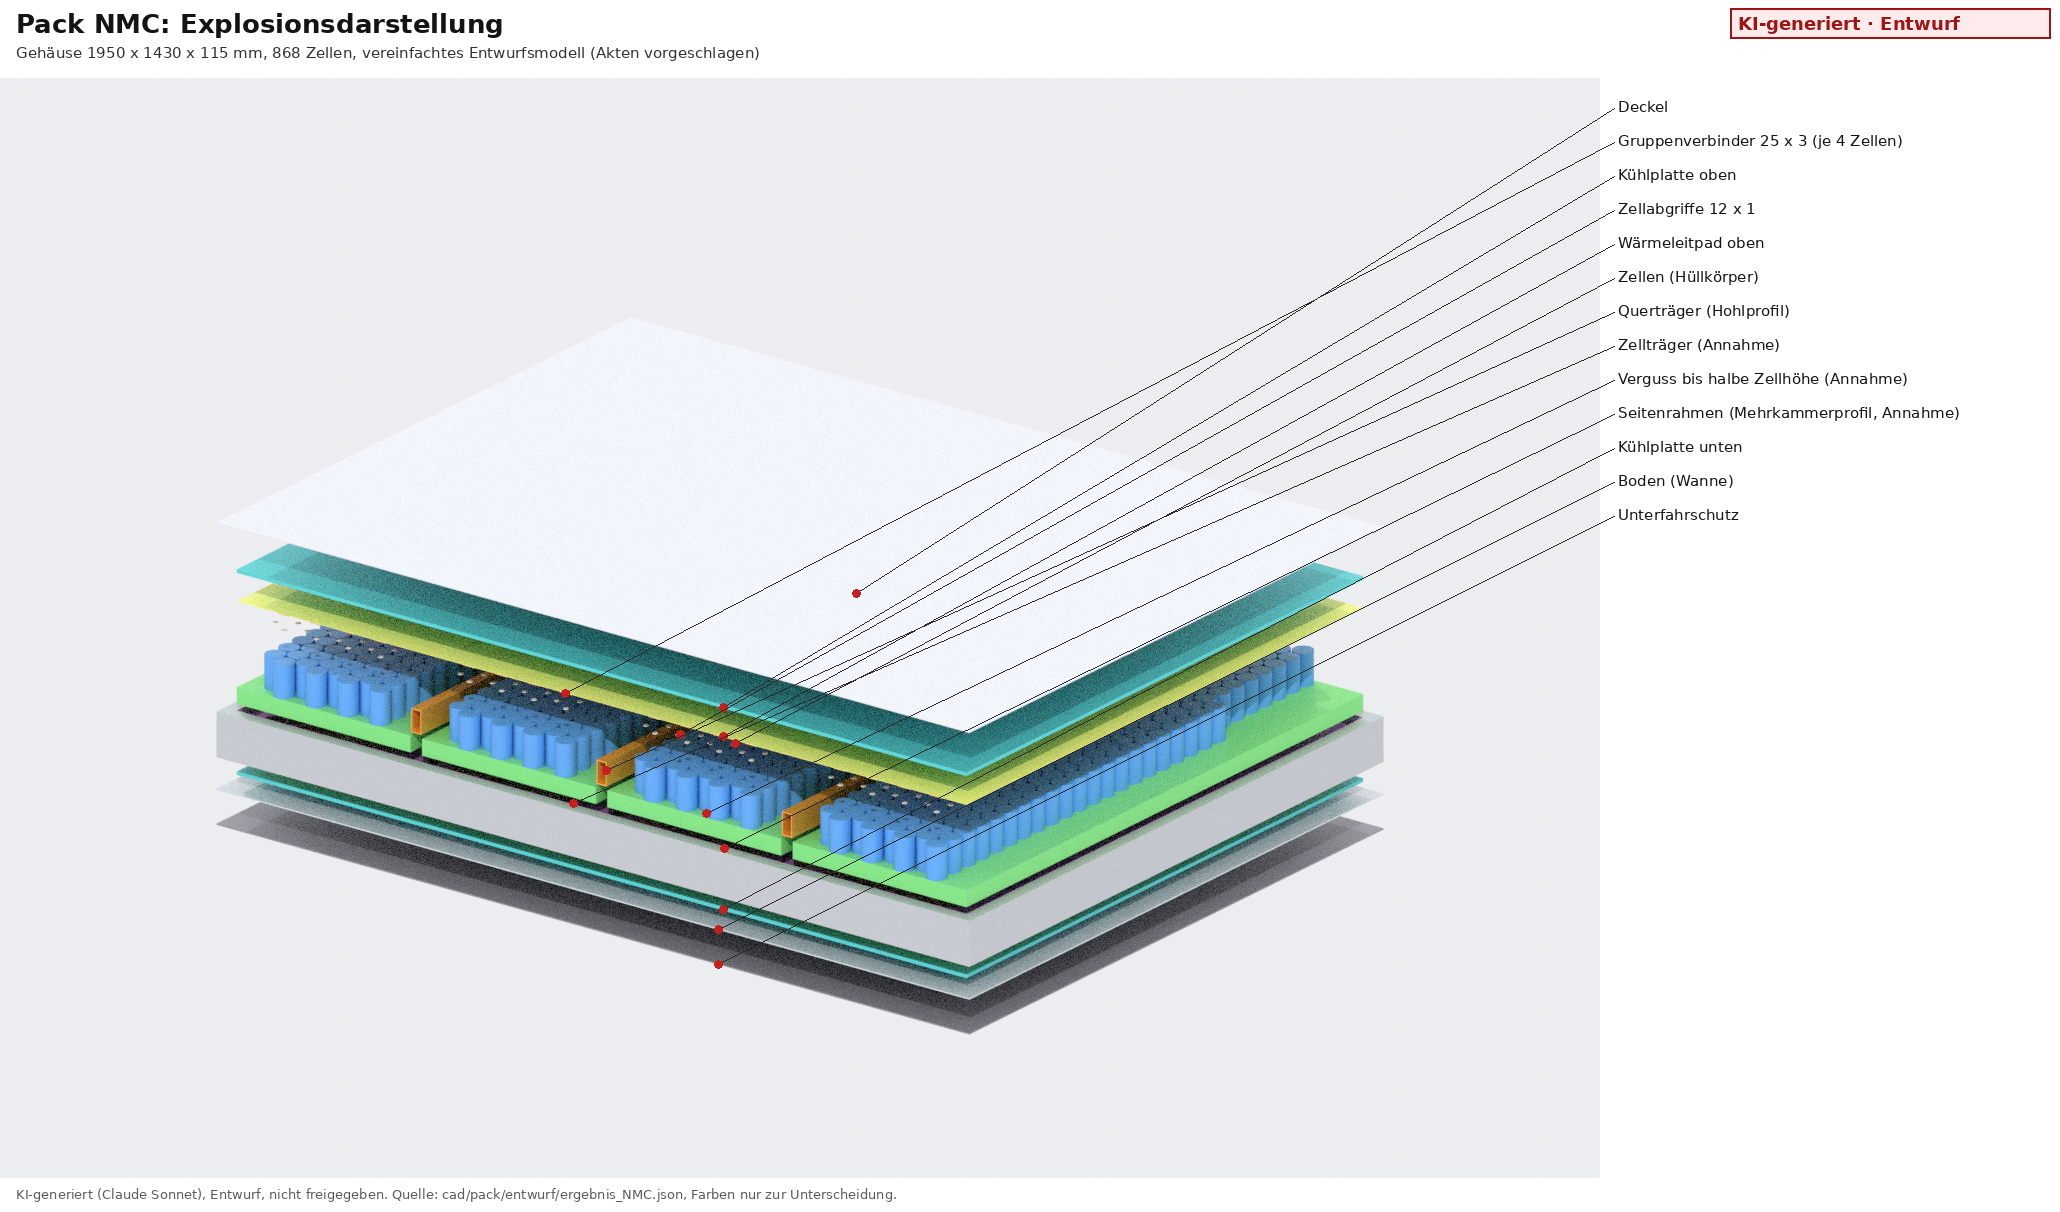
\includegraphics[width=0.49\linewidth]{bilder/g4_pack_NMC_explosion.png}
\caption[]{G4: Explosionsdarstellung LFP (links) und NMC (rechts). Quelle: \path{cad/pack/entwurf/pack_LFP_explosion.png}, \path{pack_NMC_explosion.png}.}\end{figure}
\lesehilfe{Alle Schichten auseinandergezogen, von unten nach oben: Unterfahrschutz, Boden, Kühlplatte, Pad, Zellen mit Querträgern und Verbindern, Pad, Kühlplatte, Deckel. Die Abstände sind nur Darstellung; die Linien zeigen auf das beschriftete Teil.}
\begin{figure}[H]\centering
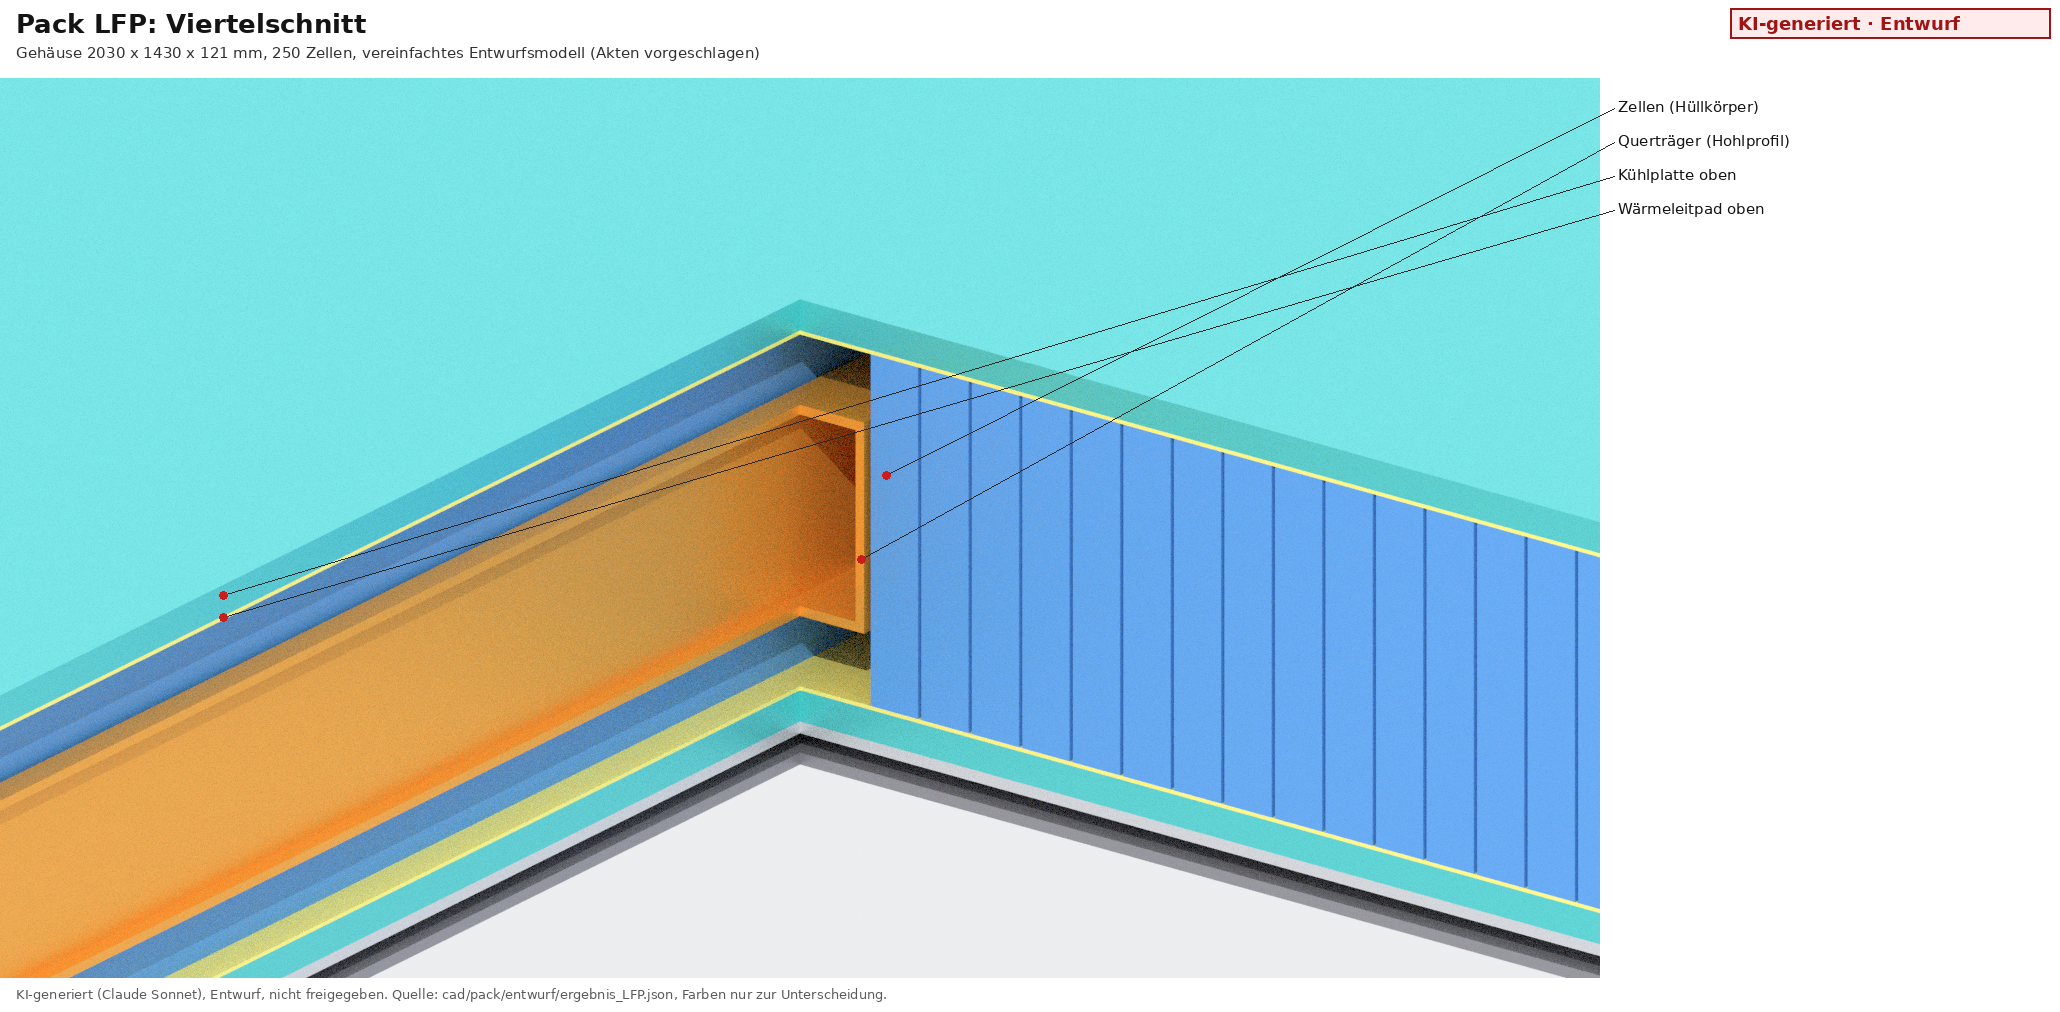
\includegraphics[width=0.49\linewidth]{bilder/g4_pack_LFP_schnitt.png}\hfill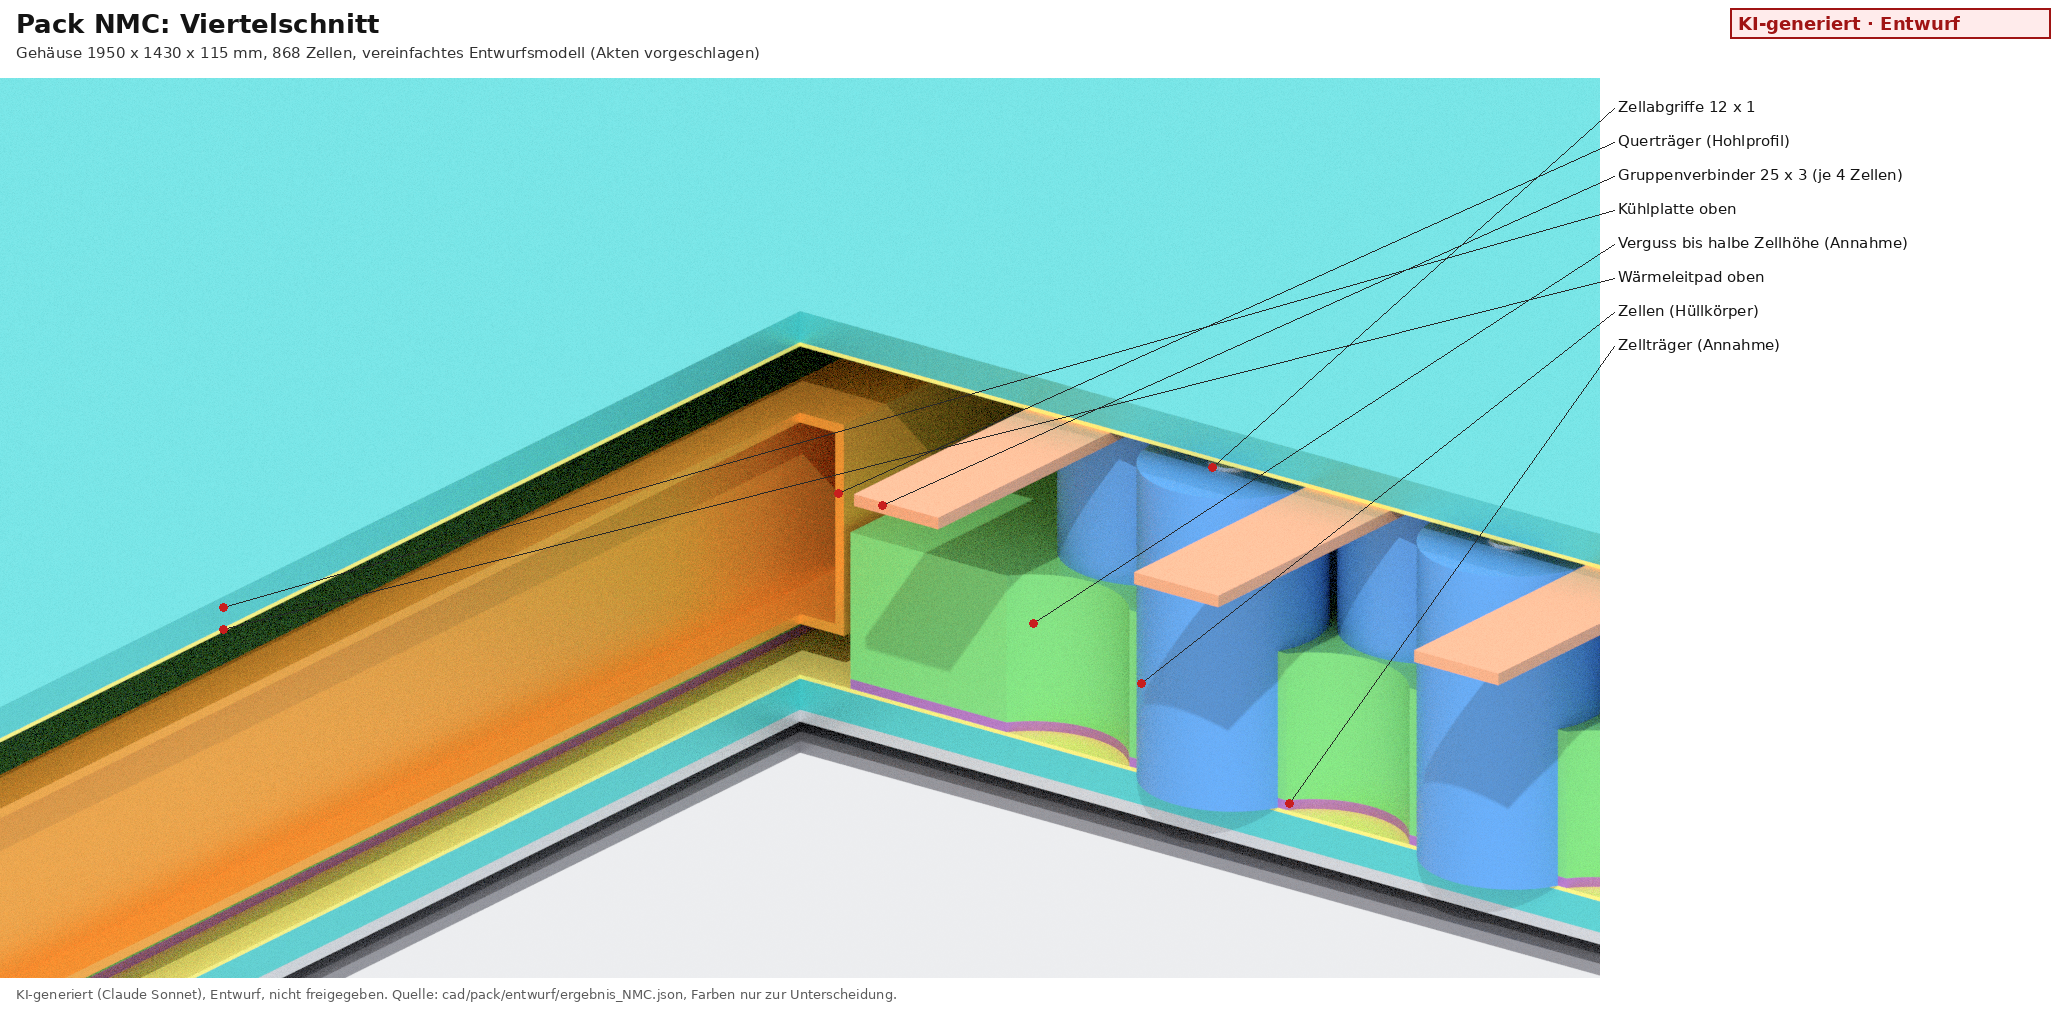
\includegraphics[width=0.49\linewidth]{bilder/g4_pack_NMC_schnitt.png}
\caption[]{G4: Viertelschnitt LFP (links) und NMC (rechts). Quelle: \path{cad/pack/entwurf/pack_LFP_schnitt.png}, \path{pack_NMC_schnitt.png}.}\end{figure}
\lesehilfe{Ein Viertel des Packs ist weggeschnitten; man sieht Zellen, Querträger und die Plattenschichten im Inneren, der Deckel ist weggelassen. Die LFP-Zellen stehen dicht an dicht zwischen den drei Querträgern, die 4680-Zellen in vier Feldern.}
\begin{figure}[H]\centering
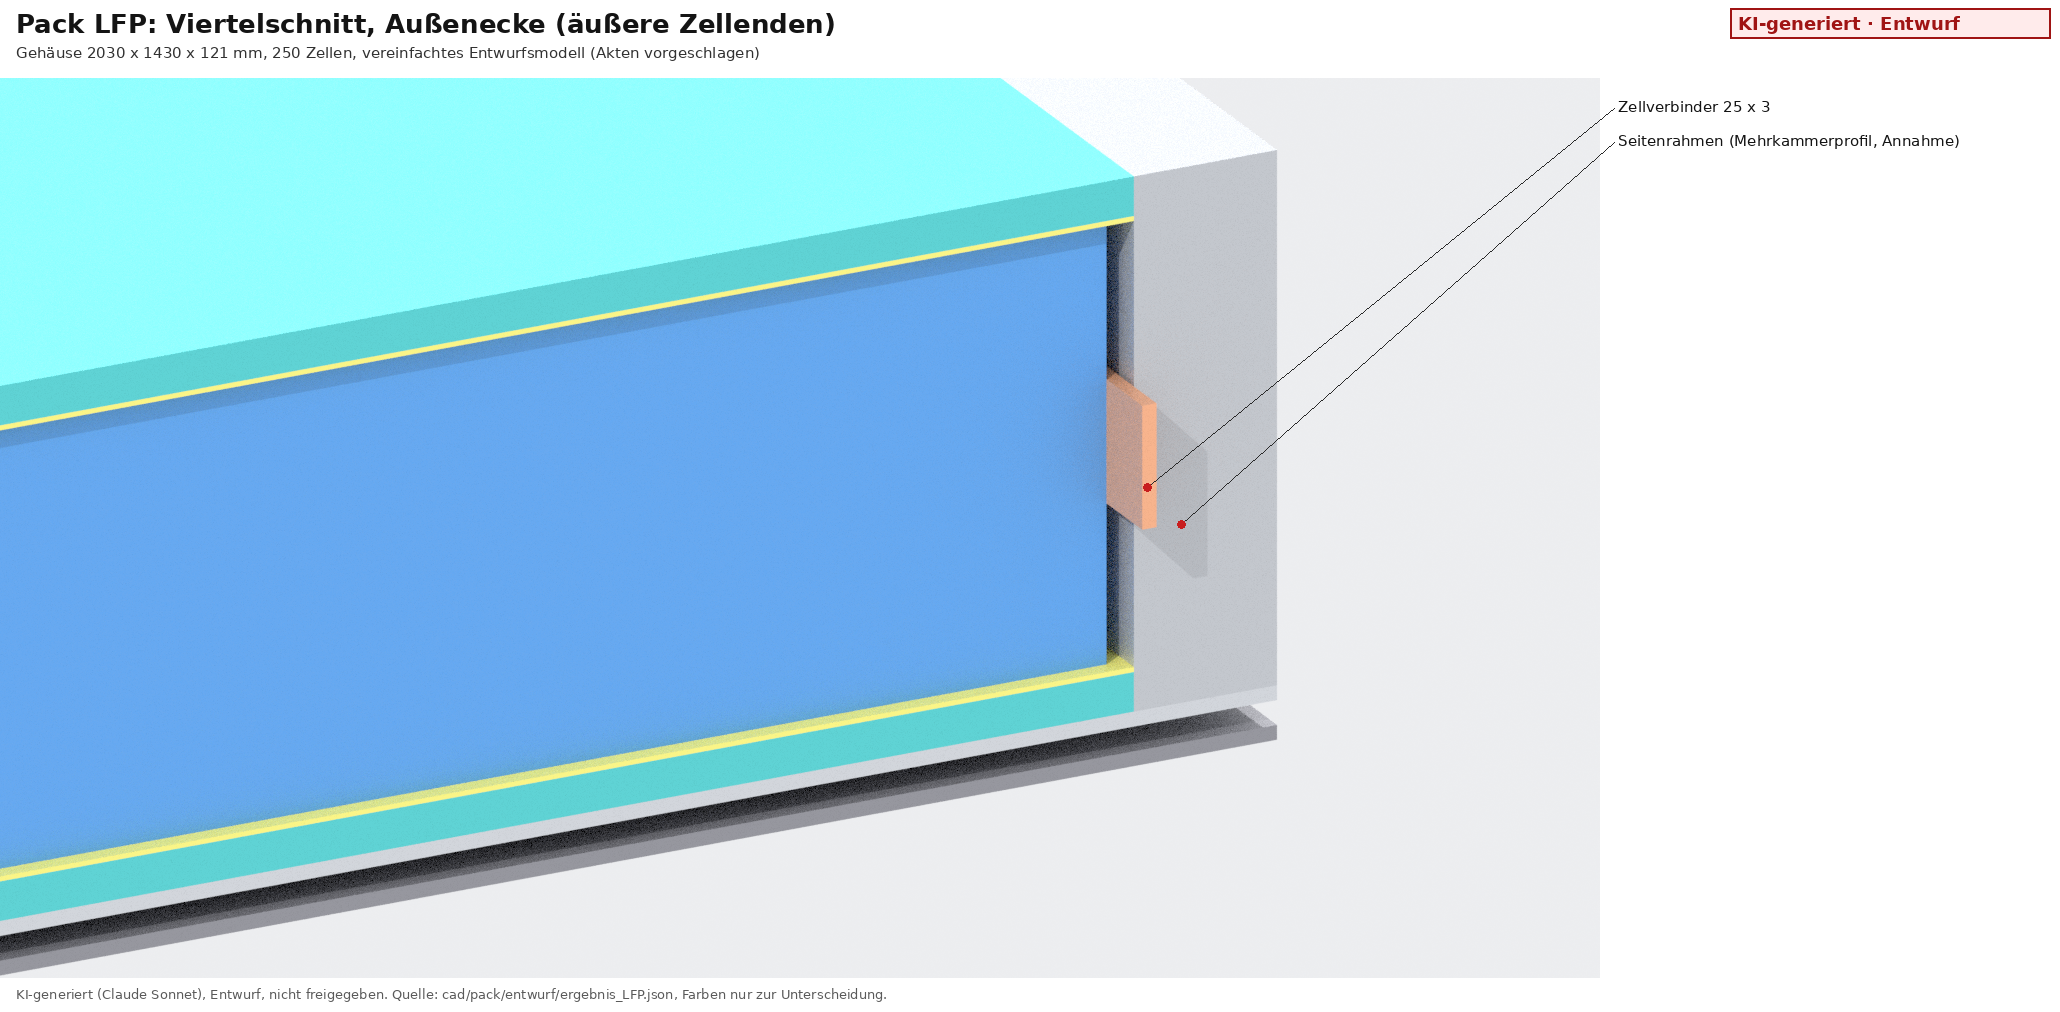
\includegraphics[width=0.49\linewidth]{bilder/g4_pack_LFP_ecke.png}\hfill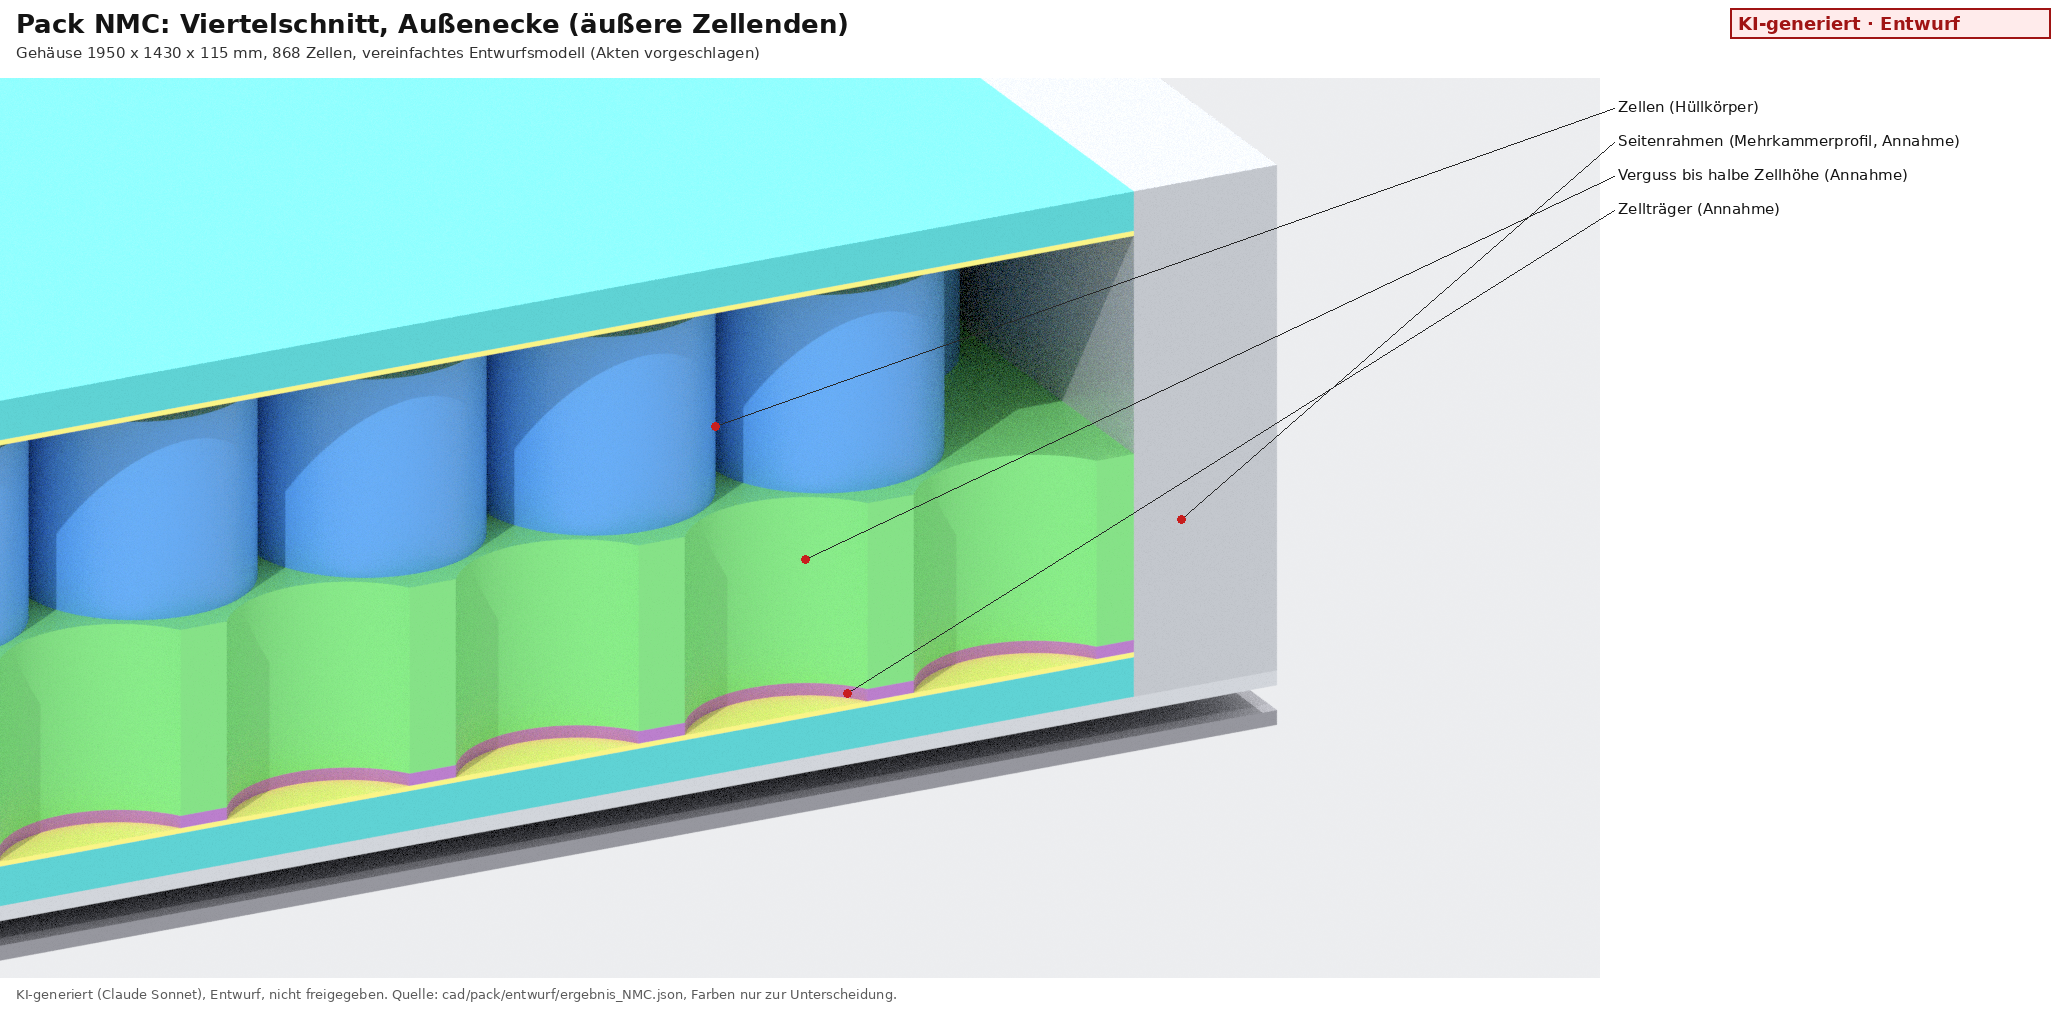
\includegraphics[width=0.49\linewidth]{bilder/g4_pack_NMC_ecke.png}
\caption[]{G4: Außenecke im Viertelschnitt, LFP (links) und NMC (rechts). Quelle: \path{cad/pack/entwurf/pack_LFP_ecke.png}, \path{pack_NMC_ecke.png}.}\end{figure}
\lesehilfe{Derselbe Viertelschnitt mit Blick auf die Schnittfläche an der Außenwand: Bei LFP sind dort die Zellverbinder (kurze Laschen am äußeren Zellende) zu sehen, bei NMC Zellträger, Verguss bis halbe Zellhöhe (Annahme), Abgriffe und Gruppenverbinder. Die Farben dienen nur der Unterscheidung.}

%======================================================================
\section{Elektrik E1: Querschnitte und Verluste}\label{k:e1}
\begriffe{\textbf{Stromdichte}: Strom je Querschnittsfläche in A/mm². \textbf{Verbinder}: Stromschiene zwischen Zellen. \textbf{HV-Hauptleitung}: Hochvolt-Leitung vom Pack zum Fahrzeug. \textbf{Spitzenstrom}: Strom über 10 s. \textbf{Verlust}: Wärme $I^2 R$ in den Leitern.}
\kasten{Stand.}{E1 ist eine Rechnung in Sekunden (CPU) aus \texttt{sim/elektrik/e1\_querschnitte/eingaben.json}. Strom aus der Last, Querschnitt aus der Stromdichte (Al ≤ 3, Cu ≤ 5 A/mm², Annahme), Erwärmung stationär gegen die Kühlplatte. Pad-Wärmeleitfähigkeit 3 W/(m·K) (Band 1 bis 5) ist \emph{nicht belegt} (Annahme).
Zahlen aus \path{sim/elektrik/e1_querschnitte/ergebnis.json}.}
\textbf{Ströme.} LFP (250s×1p): Laden 10 bis 80 \% 193,99 A, Spitze 10 s am Entladeschluss 240,0 A. NMC (217s×4p): Packstrom beim Laden 129,5 A, je Zelle 32,4 A; Spitze je Zelle am Entladeschluss 57,6 A.\quelle{\path{sim/elektrik/e1_querschnitte/ERGEBNIS.md}, Abgleich Punkt 1 und 3b; \path{ergebnis.json}, Feld \texttt{lastfaelle}}

\textbf{Gewählte Querschnitte und Verluste.}
\begin{center}\small
\begin{tabular}{@{}p{4.1cm}rrrrrr@{}}\toprule
Art & Stück & Querschnitt & J A/mm² & Verlust Dauer W & Verlust Spitze W & Masse kg\\\midrule
LFP Zell-/Reihenverbinder & 249 & Al 15×5 = 75 mm² & 2,59 & 52,8 & 80,9 & 0,76\\
LFP HV-Hauptleitung & 2 & Cu 50 mm² & 3,88 & 52,4 & 80,2 & 1,81\\
NMC Gruppenverbinder & 216 & Al 15×3 = 45 mm² & 2,88 & 254,9 & 807,0 & 6,32\\
NMC Zellabgriff & 1736 & Al 12×1 = 12 mm² & 2,70 & 98,3 & 311,3 & 1,29\\
NMC HV-Hauptleitung & 2 & Cu 35 mm² & 3,70 & 32,1 & 101,8 & 1,22\\
\bottomrule\end{tabular}\end{center}
\tquelle{\path{sim/elektrik/e1_querschnitte/ergebnis.json}, Feld \texttt{arten}; Stückzahl NMC Gruppenverbinder: 216 Reihenbrücken, dazu 217 Sammelstrecken (\path{ERGEBNIS.md}). Summen: LFP 2,57 kg und 105,2 W, NMC 8,84 kg und 385,4 W (Dauer).}

\textbf{Abgleich mit der Erwartung (Sonnet).} Erfüllt: maßgebliche Ströme, LFP-Reihenverbinder (75 mm², 249 Stück), NMC-Zellabgriff (12 mm²), HV-Hauptleitung (LFP 50 mm², NMC 35 mm²), Spannungsabfall (LFP 0,068 \%, NMC 0,442 \% bei Grenze 0,5 \%, Annahme), Erwärmung gegen die Kühlplatte (höchstens etwa 0,9 K bei $\lambda$ 1 W/(m·K), nie maßgeblich).
\emph{Verfehlt:} NMC-Gruppenverbinder 45 mm² knapp unter dem Band 50 bis 80 mm²; Verluste LFP 105,2 W (knapp über 100 W), NMC 385,4 W (über der Verfehlt-Grenze 300 W; größter Posten die Gruppenverbinder mit 254,9 W).\quelle{\path{sim/elektrik/e1_querschnitte/ERGEBNIS.md}, Abgleich Punkte 3a und 5}

\textbf{Methodenkorrektur.} Der erste Lauf setzte bei den NMC-Gruppenverbindern den vollen Gruppenstrom über die ganze Länge an (Verlust 566,3 W, Spannungsabfall 0,547 \%). Das ist konservativ, aber falsch: Der Strom wächst entlang der Sammelstrecke gleichmäßig von 0 auf $I$ (4 Zellabgriffe), der Verlust dort ist $I^2 R/3$;
nur die Reihenbrücke zur Nachbargruppe führt den vollen Strom. Nach dem Nachtrag (Annahme Opus): 385,4 W und 0,442 \%. Die Korrektur änderte die Verluste, aber nicht die Querschnittsregel.\quelle{\path{sim/elektrik/e1_querschnitte/ERGEBNIS.md}, Nachtrag Methode}
\textbf{Folge (Autor, 2026-11-17).} Der Autor hat Reihenverbinder Al 25 × 3 mm (75 mm²) für beide Varianten (ENT-096 bis 098), Zellabgriff 12 × 1 mm Al (ENT-099) und HV-Hauptleitung 50 mm² (LFP) bzw. 35 mm² (NMC) Cu (ENT-100, 101) entschieden.\quelle{\path{pm/entscheidungen/ENT-096.md} bis \path{ENT-101.md}}
E1 rechnete LFP mit 15 × 5 mm (gleicher Querschnitt 75 mm²). Eine Nachrechnung der NMC-Verluste mit dem entschiedenen Gruppenverbinder liegt nicht vor; Opus schätzte etwa 285 W (nicht gerechnet).\quelle{\path{docs/08_ki_einsatz_protokoll.md} (E1-Nachtrag-Zeile)}

\bild{e1_querschnitte.png}{0.92}{E1: gewählte Querschnitte (Dauerstrom LFP 194 A, NMC 130 A). Quelle: \path{sim/elektrik/e1_querschnitte/querschnitte.png}.}
\lesehilfe{Je Art von Stromschiene oder Kabel ein Balken mit dem gewählten Querschnitt in mm² (blau Aluminium, rot Kupfer; die Zahl darüber nennt Fläche und Breite × Dicke). Das grüne Band dahinter ist der \emph{erwartete Bereich} (Zielband). Die gestrichelte Linie ist der Querschnitt bei niedriger zulässiger Stromdichte (viel Reserve), die gepunktete der kleinste noch zulässige.
Alle Balken außer dem NMC-Gruppenverbinder (45 mm², knapp unter dem Band 50 bis 80 mm²) liegen im Band.}
\bild{e1_verluste.png}{0.92}{E1: Wärmeverlust der Verbinder je Art. Quelle: \path{sim/elektrik/e1_querschnitte/verluste.png}.}
\lesehilfe{Wärmeverlust aller Verbinder einer Art in Watt: blau bei Dauerstrom, orange bei 10 s Spitze. Das grüne Band ist das \emph{Ziel} unter 100 W, die rote Linie die Verfehlt-Grenze 300 W. LFP liegt mit gut 50 W je Art knapp im Band (Summe 105 W); bei NMC liegt der Gruppenverbinder darüber (255 W), die NMC-Summe beträgt 385 W.}

%======================================================================
\section{Fehler und Korrekturen}\label{k:fehler}
Dieses Kapitel ist der Kern für die Frage „KI im Engineering“: Wer machte welchen Fehler, wer fand ihn, wie, und was folgte. Nummern B-BAT-NNN sind Befunde in \texttt{BEFUNDE.md}.
\begin{longtable}{@{}p{0.4cm}p{3.6cm}p{2.5cm}p{4.4cm}p{3.0cm}@{}}\toprule
\textbf{Nr} & \textbf{Fehler} & \textbf{Wer machte ihn} & \textbf{Wer fand ihn, wie} & \textbf{Folge}\\\midrule\endhead
1 & NMC-Wahl in den Startwerten beruhte auf der unbelegten Annahme 180 Wh/L für LFP-Packdichte (nötig 214) & Opus (\texttt{startwerte.py}, Annahme)
 & Opus bei der Bestandsaufnahme (B-BAT-004): Recherche belegt nur Wh/kg, keinen Wert je Liter & Recherche W19/W20; Chemiewahl neu; zwei Varianten (B-BAT-004, -006)\\
2 & W06: Spalten LFP/NMC einer Tabelle vertauscht („150–220“ als LFP) & PI (lokal), Tabelle ohne Spaltengrenzen
 & Opus am Rohtext in R4; \texttt{pruefe.py} fand es nicht, weil der Wert im Text steht & Wert gesperrt (B-BAT-005)\\
3 & W19: „332 Wh/kg“ für BYD-Blade trotz bestandener Zitatprüfung (20/20) & schwache Sekundärquelle (Studentenarbeit)
 & Opus: inhaltlich unplausibel (LFP), Bezug fehlt & vier Werte gesperrt; 60 \% Volumennutzung nur als Hinweis (B-BAT-008)\\
4 & W20: PI gab die DOI statt der Datei-URL an, 0 von 21 Zitaten prüfbar & PI (DOI statt Datei-URL); der Auftrag gab die URL nicht vor
 & \texttt{pruefe.py}: 0/21; Opus ersetzte die URL, danach 17/21; Rest im Fließtext & \texttt{lauf.sh} gibt PI die Quell-URL vor (B-BAT-009)\\
5 & Zelllänge LFP 660 statt 681 mm: ENT-015 skalierte die Endzone mit der Kapazität & Opus (Akte ENT-015)
 & Opus beim Lesen von Abb. 5A: Elektrode 899,5 von 965 mm, Endzone bleibt fest (65,5 mm) & 681 mm; Bauraumbreite 1430 mm (ENT-030) (B-BAT-015)\\
6 & 4680-Wickelkern 14 statt 12,5 mm: Wickel ragte 1,15 mm über den Becher & Opus (ENT-074 nur aus der Kathodenfläche abgeleitet); zusätzlich das Modell (feste Steigung 0,45 mm auch ohne Kathode)
 & Sonnet meldete den Überstand aus dem Detailmodell; Opus fand beide Ursachen & ENT-074 auf 12,5 mm; flächentreue Spirale beauftragt (B-BAT-016)\\
7 & \texttt{stueckliste.py} las den falschen JSON-Pfad; Spannung kam still aus den Startwerten (Wert zufällig gleich) & Skript aus einem früheren Schritt (Altfehler)
 & Sonnet beim Variantenmechanismus (B-BAT-010) & Opus behob\\\midrule
8 & Werkzeug \texttt{pruefe.py}: „0 Belege“ hieß „nicht geprüft“; Zitate ohne Schlüsselwort „Beleg:“ rutschten durch & Prüfskript (Opus-Werkzeug)
 & Opus an T02/T05/T06/T08 (B-BAT-002) & jedes Zitat mit Quellenangabe geprüft\\
9 & Patente P02–P10: Spalten verrutscht (\texttt{IFS}-Tab-Fehler in \texttt{lauf.sh}) & Opus (Skript); PI blieb ehrlich (erfand nichts)
 & Opus; Google Patents antwortet danach mit HTTP 503 & Skript repariert; Patente weiter gesperrt (B-BAT-003)\\
10 & Erwartung G1 setzte die C0- statt der C0b-Energie ein (111 Ah/790 mm statt 116,2 Ah/831 mm) & Opus (Erwartung)
 & Sonnet meldete die Abweichung & Urteil „passt nicht“ unverändert (B-BAT-012)\\
11 & Erwartung K0 ohne Filmwiderstand am Kühlrand: NMC 31 statt 33,5 °C bei 1C, 45--50 statt 53,6 °C bei L2 & Opus (Erwartung)
 & gefunden durch die Rechnung; Sonnet meldete die verfehlte Erwartung, Opus fand die Ursache (Q/(h·A), 16,6 cm² Boden) & Deutung: Fehler der Erwartung, nicht der Rechnung (DEUTUNG.md)\\\midrule
12 & NMC-K3: Luftspalt statt Tab-Scheibe zwischen Wickel und Deckel (K1, erster Lauf 47,9 °C / 12,3 K) & Opus (Vorgabe: Anbindung oben nicht spezifiziert)
 & Opus bei der Deutung: Ergebnis „nicht belastbar“, real verbindet die Al-Tab-Scheibe Wickel und Deckel & Nachrechnung mit Tab-Scheibe: 38,9 °C / 5,8 K (P0), Ersatzleitfähigkeit $k_z$ 31 neue Annahme (DEUTUNG.md Punkt 4, 4a)\\
13 & E1: voller Strom über die ganze Gruppenlänge (NMC-Verlust 566,3 W) & Sonnet (Methode)
 & Opus am Band der Erwartung (Summe verfehlt) und an der Methode & Nachtrag Methode: Strom wächst entlang der Sammelstrecke, 385,4 W (E1 ERGEBNIS.md)\\
14 & G4: Massen mit Vollmaterial-Kühlplatten und -Rahmen (LFP 705,5 kg, NMC 556,5 kg) & Sonnet nach Auftrag; Massenannahmen fehlten im Auftrag (Opus)
 & Opus durch Gegenschätzung der Masse & Annahmen Füllgrad 0,4, Rahmenprofil, Dichten; 611,9 und 473,4 kg (cad/pack/ERGEBNIS.md)\\
15 & Opus-Schätzung der Ersparnis durch ein eigenes NMC-Gehäuse: 15 bis 25 kg, Ergebnis 7 kg & Opus (Schätzung ohne Rechnung)
 & G4-Rechnung (Sonnet), Opus verglich & Schätzung verworfen; Entscheidung ENT-103 steht, Wirkung gering (docs/08, G4-Zeile)\\
16 & W22: Paketgrenze 8000 Zeichen je Quelle schnitt die Maßstellen ab (Suchbegriffe zu breit; W21 ohne Maße, 12/0) & Opus (Themenliste) / Werkzeug
 & Opus an der leeren Maßtabelle von W21 & Suchbegriffe enger, Lauf 3: 13/1, Querträgermaße gefunden; SSAB „1,8 mm“ gesperrt (B-BAT, W22-Eintrag)\\
17 & Wartebefehl (Monitor) für eine Rechnung fand sich selbst statt der Rechnung & Opus (Wartebefehl)
 & Opus & Befehl neu gesetzt (Quelle: Auftrag B1-b; keine Befundnummer)\\\bottomrule
\end{longtable}
Die Zeilen 1 bis 7 sind inhaltliche Fehler im Entwurf, die Zeilen 8 bis 11 Werkzeug- und Erwartungsfehler. Neu in Fassung 0.2: Zeilen 12 und 15 Fehler in Erwartung und Vorgabe (Opus), 13 und 14 Fehler in Methode und Modell (Sonnet), 16 Recherchewerkzeug, 17 Ablauf. Das Muster: \emph{Die Prüfroutine fand formale Fehler (Wortlaut), die inhaltlichen Fehler (falsche Spalte,
unplausibler Wert, falsche Ableitung, zu große Masse) fand erst die Gegenlesung durch Opus am Rohtext, am Zielband bzw. die Rechnung.} Fehler im Werkzeug gehen nach \texttt{BEFUNDE.md}; das Modell wird nicht geändert, damit eine Zahl passt.\quelle{\path{BEFUNDE.md} B-BAT-002 bis B-BAT-016; \path{sim/kuehlung/k1_schnellladen/DEUTUNG.md}; \path{sim/elektrik/e1_querschnitte/ERGEBNIS.md}; \path{cad/pack/ERGEBNIS.md}; \path{AGENTS.md}, Grundsatz 4}

%======================================================================
\section{Entscheidungen}
Alle Akten \path{pm/entscheidungen/ENT-*.md}; Register \path{docs/04_entscheidungen.md} (erzeugt von \texttt{pm.py register}, nicht von Hand ändern). Stand: 103 Akten (ENT-001 bis ENT-103), davon 36 entschieden und 67 „vorgeschlagen“ (Zählung der Statusspalte).
\textbf{„entschieden (Mensch)“} setzt nur der Autor; „vorgeschlagen“ heißt: dem Autor vorgelegt, noch nicht entschieden.

\subsection*{Gemeinsam für beide Varianten}
\begin{longtable}{@{}p{1.6cm}p{7.0cm}p{3.8cm}p{2.0cm}@{}}\toprule
\textbf{Akte} & \textbf{Entscheidung} & \textbf{Merkmal} & \textbf{Status}\\\midrule\endhead
ENT-001 & PI recherchiert ohne Werkzeuge in drei Stufen & – & entschieden (Autor)\\
ENT-002 & Zellmodell mit PyBaMM & BT-100 & vorgeschlagen\\
ENT-003 & Opus leitet und verteilt an Sonnet, Haiku, PI & – & entschieden (Autor)\\
ENT-004 & Bauteilbaum bis Stücklistenebene, Schutzteile in Schaltbox (BT-700) & Baum & entschieden (Mensch)\\
ENT-006 & Systemspannung 800 V & BT-000 nennspannung & entschieden (Mensch)\\
ENT-012 & Baum für zwei Varianten (Zellhalter BT-250, Rundzellmaße) & Baum & entschieden (Mensch)\\
ENT-013 & Bauraumlänge 1950 mm & BT-000 bauraum\_laenge & entschieden (Mensch)\\
ENT-030 & Bauraumbreite 1430 mm & BT-000 bauraum\_breite & entschieden (Mensch)\\
ENT-031 & Bauteilbaum Innenaufbau der Zelle (BT-111 bis 116, 121, 122, 131, 132, 140) & Baum & vorgeschlagen\\
ENT-081 & Kühlart Kühlplatte unten (ersetzt durch ENT-088) & BT-600 kuehlart & entschieden (Mensch)\\
ENT-082 bis 086 & Querträger: 3 Stück quer zur Fahrtrichtung, Profil 26 × 54 mm, Wand 2,5 mm, Aluminium-Strangpressprofil & BT-530 & entschieden (Mensch)\\
ENT-087 & Seitenrahmen 30 mm je Seite & BT-540 & entschieden (Mensch)\\
ENT-088 bis 090 & Kühlart Kühlplatte oben und unten (ersetzt ENT-081), 2 Platten, Dicke 8 mm & BT-600/610 & entschieden (Mensch)\\
ENT-091 & Bauraumlänge 2030 mm für beide (ersetzt durch ENT-102) & BT-000 & entschieden (Mensch)\\
ENT-096 bis 098 & Reihenverbinder Al 25 × 3 mm (75 mm²) & BT-420 & entschieden (Mensch)\\\bottomrule
\end{longtable}
\subsection*{Variante LFP}
\begin{longtable}{@{}p{1.9cm}p{7.2cm}p{3.5cm}p{2.0cm}@{}}\toprule
\textbf{Akte} & \textbf{Entscheidung} & \textbf{Merkmal} & \textbf{Status}\\\midrule\endhead
ENT-005 & Zellchemie LFP (Blade-Format) als Hauptvariante & BT-100 chemie & entschieden (Mensch)\\
ENT-014 bis 020 & Zellformat, Länge 681 mm, Breite 90 mm, Dicke 14 mm, 92,4 Ah, 3,2 V, 1850 g & BT-100 & vorgeschlagen\\
ENT-021, 022 & Z-gefalteter Stapel, 38 Kathodenlagen & BT-110 & vorgeschlagen\\
ENT-023, 024 & Gehäuse Aluminium, Wand 0,3 mm & BT-120 & vorgeschlagen\\
ENT-032 bis 056 & Innenaufbau: Elektroden, Separator, Isolierrand, Fixierung, Gehäusefolie, Füllöffnung, Stromschiene, Fügeverfahren, Polisolation, Ventil & BT-111 bis 140 & vorgeschlagen\\
ENT-100 & HV-Hauptleitung 50 mm² Cu & BT-430 & entschieden (Mensch)\\
ENT-102 & Bauraumlänge 2030 mm, eigenes Gehäuse (ersetzt ENT-091) & BT-000 & entschieden (Mensch)\\\bottomrule
\end{longtable}
\subsection*{Variante NMC}
\begin{longtable}{@{}p{1.9cm}p{7.2cm}p{3.5cm}p{2.0cm}@{}}\toprule
\textbf{Akte} & \textbf{Entscheidung} & \textbf{Merkmal} & \textbf{Status}\\\midrule\endhead
ENT-007 bis 011 & NMC811, Rundzelle 4680, 23,125 Ah, 3,7 V, 355 g (Wahl des Autors, Werte W20) & BT-100 & entschieden (Mensch)\\
ENT-025, 026 & Durchmesser 46 mm, Höhe 80 mm & BT-100 & vorgeschlagen\\
ENT-027 bis 029 & Wickel (tabless), Stahlgehäuse, Wand 0,4 mm & BT-110, BT-120 & vorgeschlagen\\
ENT-057 bis 080 & Innenaufbau: Bänder, Kern Ø 12,5 mm (ENT-074), Fixierung, Blindniet, Tab-Scheiben, Fügeverfahren, Polisolation, Ventil im Boden & BT-111 bis 140 & vorgeschlagen\\
ENT-092 bis 095 & Zellhalter Kunststoffträger unten plus Verguss; Zellverbinder oben Al, Laserschweißen; isolierende Wärmeleitschicht oben & BT-250, BT-410, BT-230 & entschieden (Mensch)\\
ENT-099 & Zellabgriff 12 × 1 mm Al & BT-410 & entschieden (Mensch)\\
ENT-101 & HV-Hauptleitung 35 mm² Cu & BT-430 & entschieden (Mensch)\\
ENT-103 & Bauraumlänge 1950 mm, eigenes Gehäuse & BT-000 & entschieden (Mensch)\\\bottomrule
\end{longtable}

%======================================================================
\section{Offene Punkte und nächste Schritte}\label{k:offen}
\begin{itemize}[nosep]
\item \textbf{Freigaben:} etwa 30 vorgeschlagene Werte je Variante (Zellmaße und Innenaufbau, ENT-014 bis ENT-080), dazu ENT-002 (PyBaMM) und ENT-031 (Baum Innenaufbau); insgesamt 67 Akten im Status „vorgeschlagen“.\quelle{\path{docs/04_entscheidungen.md}}
\item \textbf{Polmaße und Fahnen-Lesart:} Polgrößen sind Annahmen; die Bedeutung der Fahnenmaße in W20 Abb. 5A (LFP 27,1/9 und 20,5/7 mm; 4680 2,5/5 und 7,5/2,5 mm) ist offen. Isolierrand und Klebeband sind nicht modelliert.
\item \textbf{Kühlplatte BT-610, Kanäle:} Kanalgeometrie und Strömung (FluidX3D) sind nicht gerechnet; der Füllgrad 0,4 der Massenrechnung und $h$ 500 W/(m²·K) sind Annahmen.
\item \textbf{Crash und Festigkeit (X):} Seitencrash quasistatisch (CalculiX) fehlt; die Seitenlast 600 kN aus W22 gilt für Fahrzeuge über 2600 kg, der Lastfall für 1500 kg ist offen (Autor-Frage aus M0). Seitenrahmenprofil (Wand 2,5 mm, 3 Kammern) ist Annahme Opus.
\item \textbf{Zellmodell C1 bis C3} (PyBaMM): Eichung des Innenwiderstands am Blade-Pulsdatensatz (Borealis, CC-BY 4.0, BYD Blade 135 Ah, 10-s-Pulse, $-10$ bis 40 °C). Der Innenwiderstand ist die stärkste Annahme der Wärmerechnung.
\item \textbf{Bericht EN} (englische Fassung), Schlussbericht, Video und Präsentation.
\item \textbf{NMC-Masse:} 473,4 kg verfehlt das Zielband 390 bis 430 kg ($+15{,}2$ \% gegen C0b); Deutung offen (Opus).
\item \textbf{NMC-Verluste Elektrik:} 385,4 W über der Verfehlt-Grenze 300 W; Nachrechnung mit dem entschiedenen Gruppenverbinder (25 × 3 mm) fehlt. LFP 105,2 W knapp über 100 W.
\item \textbf{K1b:} Annahmen zum oberen Kühlpfad der 4680 ($\varphi$ 0,5, Pad $k$ 3 W/(m·K), 1 mm); Opus-Deutung steht aus. Ebenso die Spaltleitfähigkeit $k_z$ 31 W/(m·K) der Tab-Scheibe (K3).
\item \textbf{Zahlenabweichung in \path{sim/kuehlung/TABELLEN_TEMPERATUR.md}:} Die K1-Tabelle der Sammeldatei enthält für die 4680 teils Werte des alten Netzes (z. B. P0 53,6 °C / 16,0 K gegen 53,4 °C / 15,7 K in \path{ergebnis.json}, P3 mit K1b 36,9 / 5,5 gegen 36,8 / 5,4). Dieser Bericht verwendet \path{ergebnis.json}; die Sammeldatei ist nachzuziehen (Opus).
\item \textbf{Gehäusewand 4680:} Akte ENT-029 setzt 0,4 mm (W20 Tab. 1), W24 und W25 nennen 0,5 bis 0,6 mm für die Tesla-4680; welche Zahl gilt, ist offen.
\item \textbf{Zielband Masse in Fall B:} Die Empfindlichkeitsgrafik nennt für LFP Fall B als 30-\%-Grenze 683 kg, die Kriterientabelle 644 kg. Welche Zahl gilt, ist ungeklärt (Opus prüft); der Bericht verwendet keine der beiden.\quelle{\path{sim/chemie/varianten_lfp_nmc/empfindlichkeit.png}, \path{kriterien.png}}
\item \textbf{Verschaltung G3} (BMS-Kanäle, Zellverbinder-Kontaktwiderstand) und \textbf{Zellhalter} im Detail; NMC-Zellträger 2,5 mm ist Platzhalter (Annahme).
\item \textbf{Offene Lastenheft-Punkte:} Leistung (REQ-P04), Umgebung (P08), Lebensdauer (P10), Sicherheit (P11), Kühlmittel (P12) und weitere; Fall A oder B (1500 kg mit oder ohne Batterie) bleibt ein Anhaltswert.
\item \textbf{Schwache Annahmen mit Wirkung:} Volumennutzung 60 \% (Sekundärquelle, kippt LFP Fall A), Zellabstand 1 mm und Rand 30 mm, Packfaktor 0,75.
\end{itemize}

%======================================================================
\appendix
\section*{Anhang A: Begriffe (Glossar)}
\addcontentsline{toc}{section}{Anhang A: Begriffe (Glossar)}
\begin{tabularx}{\linewidth}{@{}lX@{}}\toprule
Anode / Kathode & Minus- bzw. Pluselektrode einer Zelle.\\
Akte (ENT) & Entscheidungsdokument mit Wert, Begründung, Belegen, Status.\\
Annahme & Wert ohne Beleg; wird im Dokument so benannt.\\
BMS & Batteriemanagementsystem (Spannung, Temperatur, Schutz).\\
Fall A / Fall B & 1500 kg mit bzw. ohne Batterie.\\
G1 / G2 / G3 / G4 & Vorgänge: Zellanordnung im Bauraum / Zell-CAD / Verschaltung / Pack.\\
K0 & Wärmesimulation einer Zelle je Variante.\\
Kühlplatte & flache Platte mit Kühlmittelkanälen unter den Zellen.\\
LFP / NMC & Lithium-Eisenphosphat / Nickel-Mangan-Kobalt-Oxid.\\
orthotrop & Eigenschaft hängt von der Richtung ab (z. B. Wärmeleitung).\\
Packfaktor k & Anteil der Zellmasse an der Packmasse.\\
Separator & poröse Trennfolie zwischen Anode und Kathode.\\
tabless & ohne einzelne Anschlussfahnen.\\
Volumennutzung & Anteil des Packvolumens, der Zelle ist.\\
Wickel (jelly roll) & zur Spirale gerollte Elektroden.\\
Z-Faltung & Ziehharmonika-Faltung des Separators.\\\bottomrule
\end{tabularx}

\section*{Anhang B: Quellen}
\addcontentsline{toc}{section}{Anhang B: Quellen}
Recherche-Themen (\path{forschung/themen_wissen.tsv}); die Texte selbst liegen nicht im Repository.
\begin{itemize}[nosep]
\item W01 LFP: \url{https://en.wikipedia.org/wiki/Lithium_iron_phosphate_battery}
\item W03 BYD Blade: \url{https://en.wikipedia.org/wiki/Blade_battery}
\item W06 Elektrofahrzeug-Batterie: \url{https://en.wikipedia.org/wiki/Electric_vehicle_battery}
\item W10 NMC, LTO: \url{https://en.wikipedia.org/wiki/Lithium_nickel_manganese_cobalt_oxides}
\item W12 Batteriepack, CCS: \url{https://en.wikipedia.org/wiki/Battery_pack}
\item W16 Thermomanagement: \url{https://en.wikipedia.org/wiki/Battery_thermal_management}
\item W17 Seitencrash: \url{https://en.wikipedia.org/wiki/Side_collision}
\item W18 314-Ah-LFP-Zelle, thermische Kennwerte: \url{https://www.techscience.com/fhmt/online/detail/29043/TSP_FHMT_92550.pdf}
\item W19 Blade-Zelle (Sekundärquelle, teils gesperrt): \url{https://drpress.org/ojs/index.php/HSET/article/download/5087/4928}
\item W20 Zerlegungsstudie BYD Blade gegen Tesla 4680, Cell Reports Physical Science 6, 102453 (2025), doi:10.1016/j.xcrp.2025.102453, \textbf{Lizenz CC-BY}; PDF vom Autor in \path{quellen/blade_zerlegung/}, nicht im Repository.
\item Pulsdatensatz „Battery State-of-power Measurement“, Borealis, doi:10.5683/SP3/RPCWBY, CC-BY 4.0 (für C2/C3 vorgesehen).
\end{itemize}
Lizenzliste: \path{docs/10_lizenzen_und_quellen.md}.

\section*{Anhang C: Software}
\addcontentsline{toc}{section}{Anhang C: Software}
Versionen laut \path{SOFTWARE.md} (Stand 2026-11-11): FreeCAD 1.1.4 (AppImage, headless); Blender 4.0.2 (Render, Cycles auf der CPU); ElmerFEM 26.2; gmsh 4.12.1 (System) bzw. 4.15.2 (Python);
PyBaMM 26.10.1.1; ParaView (System); CalculiX 2.21; pdflatex (System). Lokaler Agent: PI mit ollama \texttt{qwen-gross} (27B, 64k), ohne Werkzeuge. Python-Umgebung \texttt{.venv}
(\path{requirements.txt}).

\vfill
\kigen{Dokument BAT-DOC-17, Version 0.1, Status Entwurf, Ersteller Claude Opus/Sonnet. Nicht vom Menschen freigegeben. Fassung EN folgt.}
\end{document}
